
\chapter{Apparatus}
\label{chap:apparatus}

%\chapterquote{This thing, what is it in itself, in its own constitution? What is its substance and material?}{Marcus Aurelius}


\section{Introduction}
This chapter describes the experimental apparatus used to produce the 2016 proton-proton collision dataset used in this thesis. A description of the means of collision production, the Large Hadron Collider (LHC), will be given and their measurement with the Compact Muon Solenoid (CMS) will be described in particular detail. The CMS design and operation described here will correspond to the 2016 running period.

\section{The Large Hadron Collider}
The LHC \cite{LHC_design_report} is a large synchrotron-type particle accelerator whose purpose is to provide collisions to survey electroweak-scale physics, particularly the mechanism of electroweak symmetry breaking, in addition to a broad physics program ranging from dark matter searches to flavour physics to studies of quark-gluon plasma.
These studies are afforded by the production of high-energy and high-luminosity proton and lead ion collisions in counter-circulating beams. These achieve a long reach for the production of heavy particles and superior statistical power for the study of rare processes. 
The remainder of this section will be solely concerned with the LHC's proton-proton operation.  

\subsection{LHC Accelerator Chain}

Before collisions occur at the LHC interaction points the beams must be produced and conditioned with a collection of accelerators \cite{CERN_accelerator_complex} before injection into the LHC (Figure \ref{fig:apparatus:lhc_chain}).
\begin{figure}[h!]
    \centering
    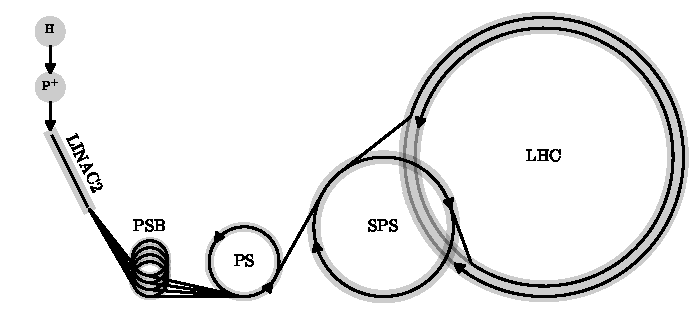
\includegraphics[width=0.9\textwidth]{figures/apparatus/accel_chain.pdf}
    \caption{A schematic view of the LHC accelerator chain for proton-proton operation.}
    \label{fig:apparatus:lhc_chain}
\end{figure}
This process begins with the acquisition of protons from a small quantity of hydrogen gas: hydrogen is injected into a chamber and the atomic electrons are stripped off using a strong electric field. The resulting bare protons are then injected into a linear accelerator (LINAC 2) and accelerated by radiofrequency (RF) cavities to an energy of 50\,MeV. The protons then enter the Proton Synchrotron Booster (PSB), consisting of four synchrotron rings stacked on top of each other with a radius of 25\,m, the protons are further accelerated up to an energy of 1.4\,GeV allowing for more protons to be injected into the next part of the accelerator chain and therefore higher-intensity beams.
The protons from each ring of the PSB enter the Proton Synchrotron (PS) in sequence with 25\,ns spacing to form the bunch structure. The PS is another synchrotron with a radius of 72\,m where they are accelerated to 25\,GeV. 
When they have reached this energy the protons are then injected into the Super Proton Synchrotron (SPS) which has a circumference of nearly 7\,km and accelerates protons to 450\,GeV before their injection into the LHC in two opposing directions. 


\subsection{LHC Structure and Operation}
The LHC itself is a 27\,km ring consisting of 1232 8\,T superconducting dipole magnets that force the protons into a circular path so they can be repeatedly accelerated by 16 superconducting RF cavities oscillating at 400\,MHz. As on-time protons with correct energy come in to the cavity they do not experience any acceleration, if they arrive slightly later they experience an accelerating potential, slightly early and they experience a deceleration. This maintains the energy of the protons and the bunch structure as they circulate in the LHC ring. The beams are then further adjusted by 392 quadrupole magnets to maintain stable beam conditions and stronger quadrupole magnets are used to focus the beams at the four LHC collision points.

Bunches of protons are brought together to collide at each of the LHC interaction points every 25\,ns during normal operation. This is referred to as a bunch crossing and usually produces multiple superimposed proton collisions (pileup) and a large dose of radiation for any equipment situated nearby. These conditions pose challenges for the design and operation of the LHC's experiments. 

The LHC is designed to operate with a centre of mass energy of $\sqrt{s}=14$\,TeV and instantaneous luminosity of $10^{34}$\,$\mathrm{cm}^{-2}\mathrm{s}^{-1}$ with two beams of 2880 bunches. During the 2016 period the LHC operated at $\sqrt{s} = 13$\,TeV and an instantaneous luminosity above design specification at $1.4\times{}10^{34}$\,$\mathrm{cm}^{-2}\mathrm{s}^{-1}$. This culminated in 40.82\,fb$^{-1}$ of integrated luminosity delivered to the CMS experiment in the 2016 period with an average pileup rate of 27 \cite{CMSLumiPublic} (Figure \ref{fig:apparatus:cms_int_lumi}).
\begin{figure}[h!]
    \begin{center}
    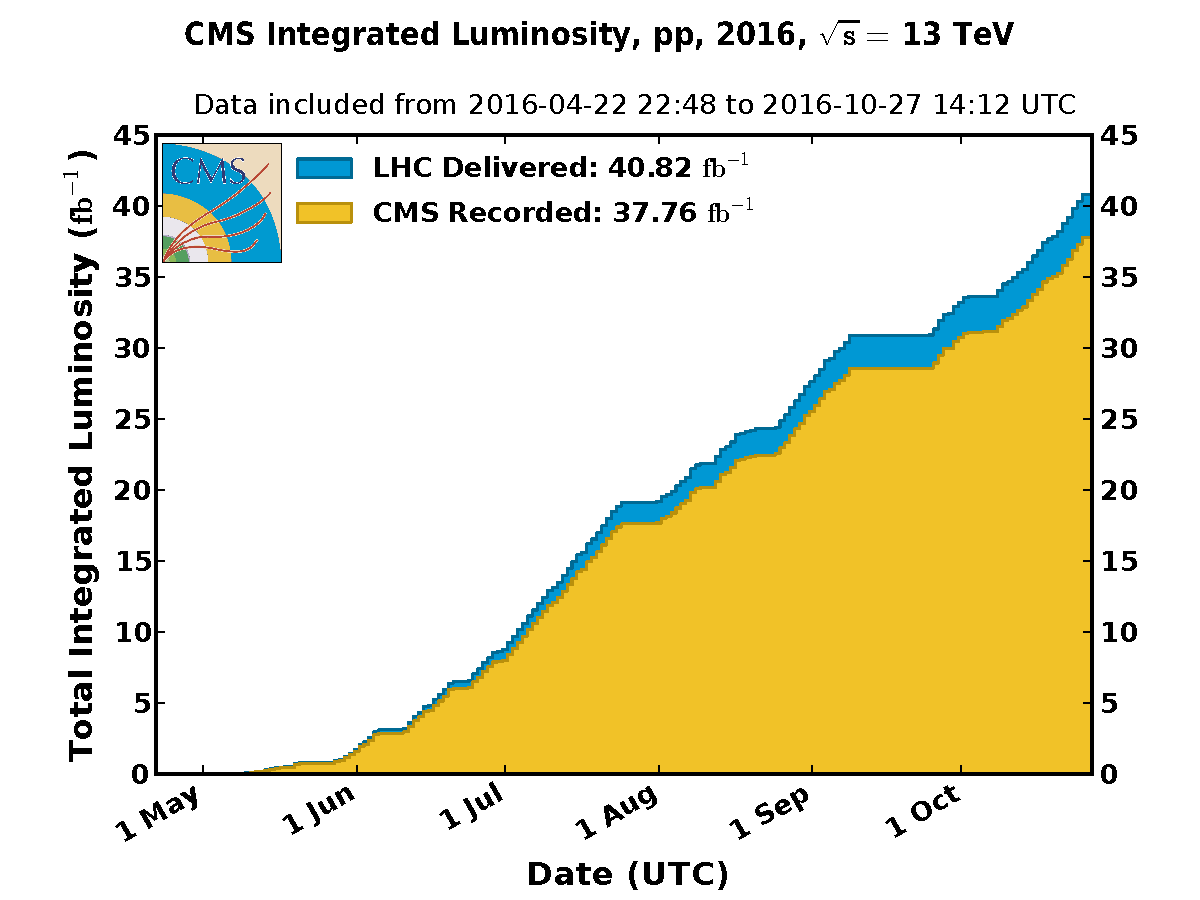
\includegraphics[width=0.49\textwidth]{figures/apparatus/int_lumi_per_day_cumulative_pp_2016.pdf}
    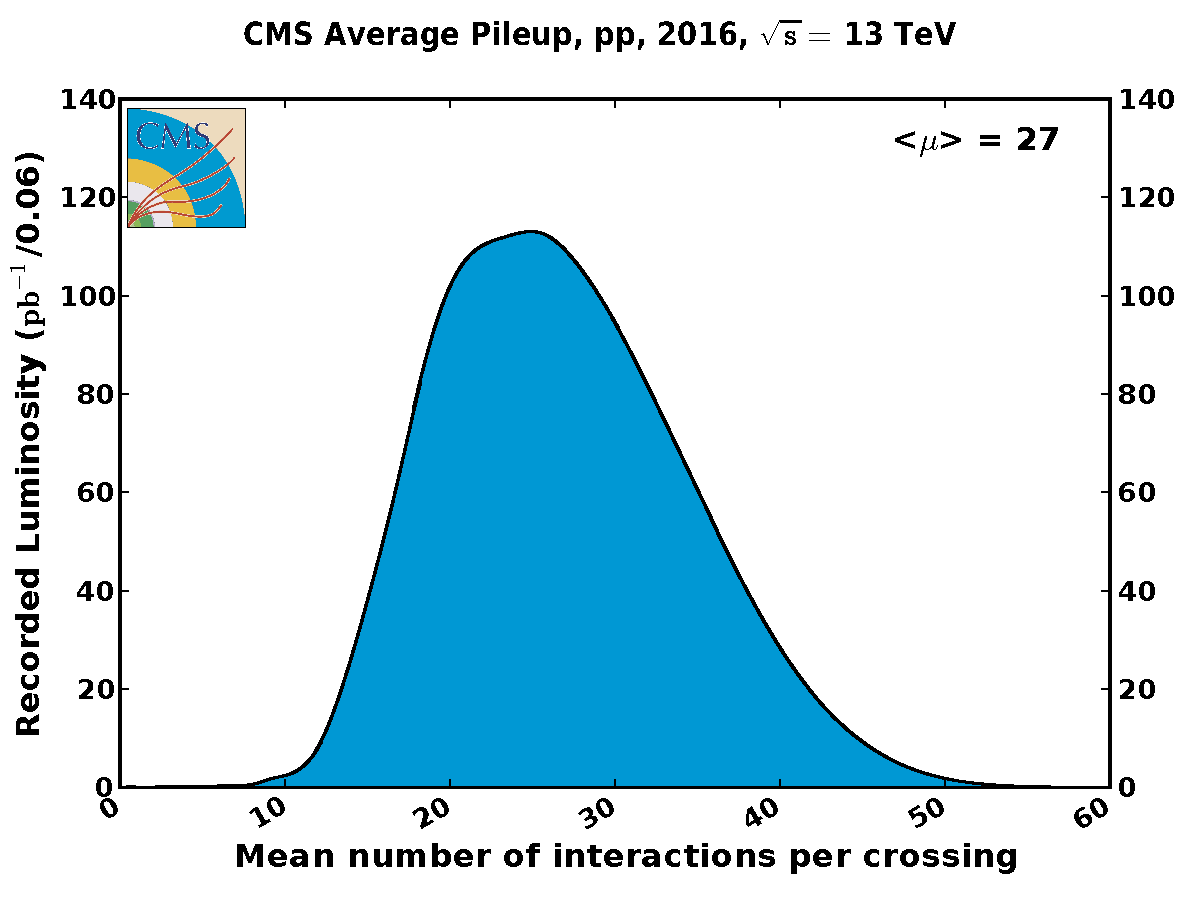
\includegraphics[width=0.49\textwidth]{figures/apparatus/pileup_pp_2016.pdf}
    \end{center}
    \caption{Left: total integrated luminosity over the 2016 proton-proton running period delivered to (blue) and recorded by (orange) the CMS experiment \cite{CMSLumiPublic}. Right: the 2016 pileup distribution \cite{CMSLumiPublic}.}
    \label{fig:apparatus:cms_int_lumi}
\end{figure}


\section{The Compact Muon Solenoid}

The CMS experiment \cite{CMSatLHC} is a general-purpose detector situated at Point 5 on the LHC directly opposite its counterpart, ATLAS \cite{AtlasatLHC}. CMS uses a right-handed coordinate system with the $x$-axis pointing horizontally towards the centre of the ring, the $y$-axis pointing vertically, and the $z$-axis pointing along the beamline in the anti-clockwise direction. 
An angular coordinate system is commonly used in physics analyses which consists of the coordinates $(\phi,\eta,z)$, where $\phi$ is the azimuthal angle in the $x$-$y$ plane and $\eta$ is the pseudorapidity defined from the polar angle $\theta$ as
\begin{equation}
    \label{eq:apparatus:pseudorapidity}
    \eta = -\ln\tan{\frac{\theta}{2}}.
\end{equation}
Generally, the high $|\eta|$ regions closer to the beamline are referred to as forward, and the low $|\eta|$ region is referred to as central. 
In addition, the radial distance in the $x$, $y$ plane $r$ is sometimes used. The different coordinates used at CMS are summarised in Figure \ref{fig:apparatus:coords}. This thesis will use the $(\phi,\eta,z)$ coordinate system. 
\begin{figure}[h!]
    \centering
    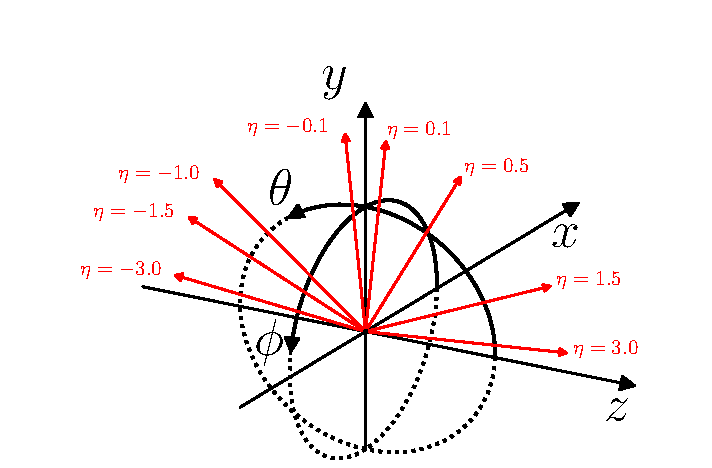
\includegraphics[width=0.45\textwidth]{figures/apparatus/CMS_coords.pdf}
    \caption{Coordinate systems used at CMS. Example values for the pseudorapidity $\eta$ are shown by the red arrows.}
    \label{fig:apparatus:coords}
\end{figure}

\subsection{Design Overview}
The design of CMS is driven by the challenges of operating in the LHC collision environment and by the broad range of its physics goals \cite{CMSPhysics}.
The LHC produces proton-proton bunch crossings at a high rate (40\,MHz) and this requires CMS to be very responsive to facilitate a short decision time on accepting an event. This high collision rate also means that the components of CMS operate in a high-radiation environment, so their performance must be robust to large doses of radiation. Finally, the pileup in each bunch crossing puts particular requirements on the CMS design to achieve isolation of different kinds of particles in a complex, high-multiplicity environment: it requires fine granularity, both spatial and temporal. 


The physics goals of CMS include the discovery and measurement of the Higgs boson and searches for supersymmetry amongst other topics like extra gauge bosons, extra dimensions and heavy ion collisions. 
The CMS Higgs physics programme has prioritised searches for the Higgs boson in the leptonic final states as well as the diphoton final state as these have superior signal separation potential and mass resolution in the LHC collision environment when compared to hadronic searches. For supersymmetry searches one expects events with a significant degree of missing-transverse energy ($E_{T}^{\mathrm{miss}}$) and this, along with maximising the acceptance of other analyses, motivates the hermetic design of CMS. Therefore, the main CMS performance goals were decided to be \cite{CMSatLHC}:
\begin{itemize}[noitemsep]%[leftmargin=.5in,noitemsep]
    \item Good identification of muons and good muon momentum resolution,
    \item Good charged particle momentum resolution and reconstruction efficiency,
    \item Efficient triggering and offline tagging for $\tau$ leptons and $b$ quark jets, 
    \item Good energy resolution for electromagnetically interacting particles over a large geometric area, and $\pi^{0}$ rejection,
    \item Good missing-transverse energy and dijet mass resolution.
\end{itemize}
The design of CMS, shown in Figure \ref{fig:apparatus:CMS}, is driven by these goals. 
\begin{figure}[h!]
%    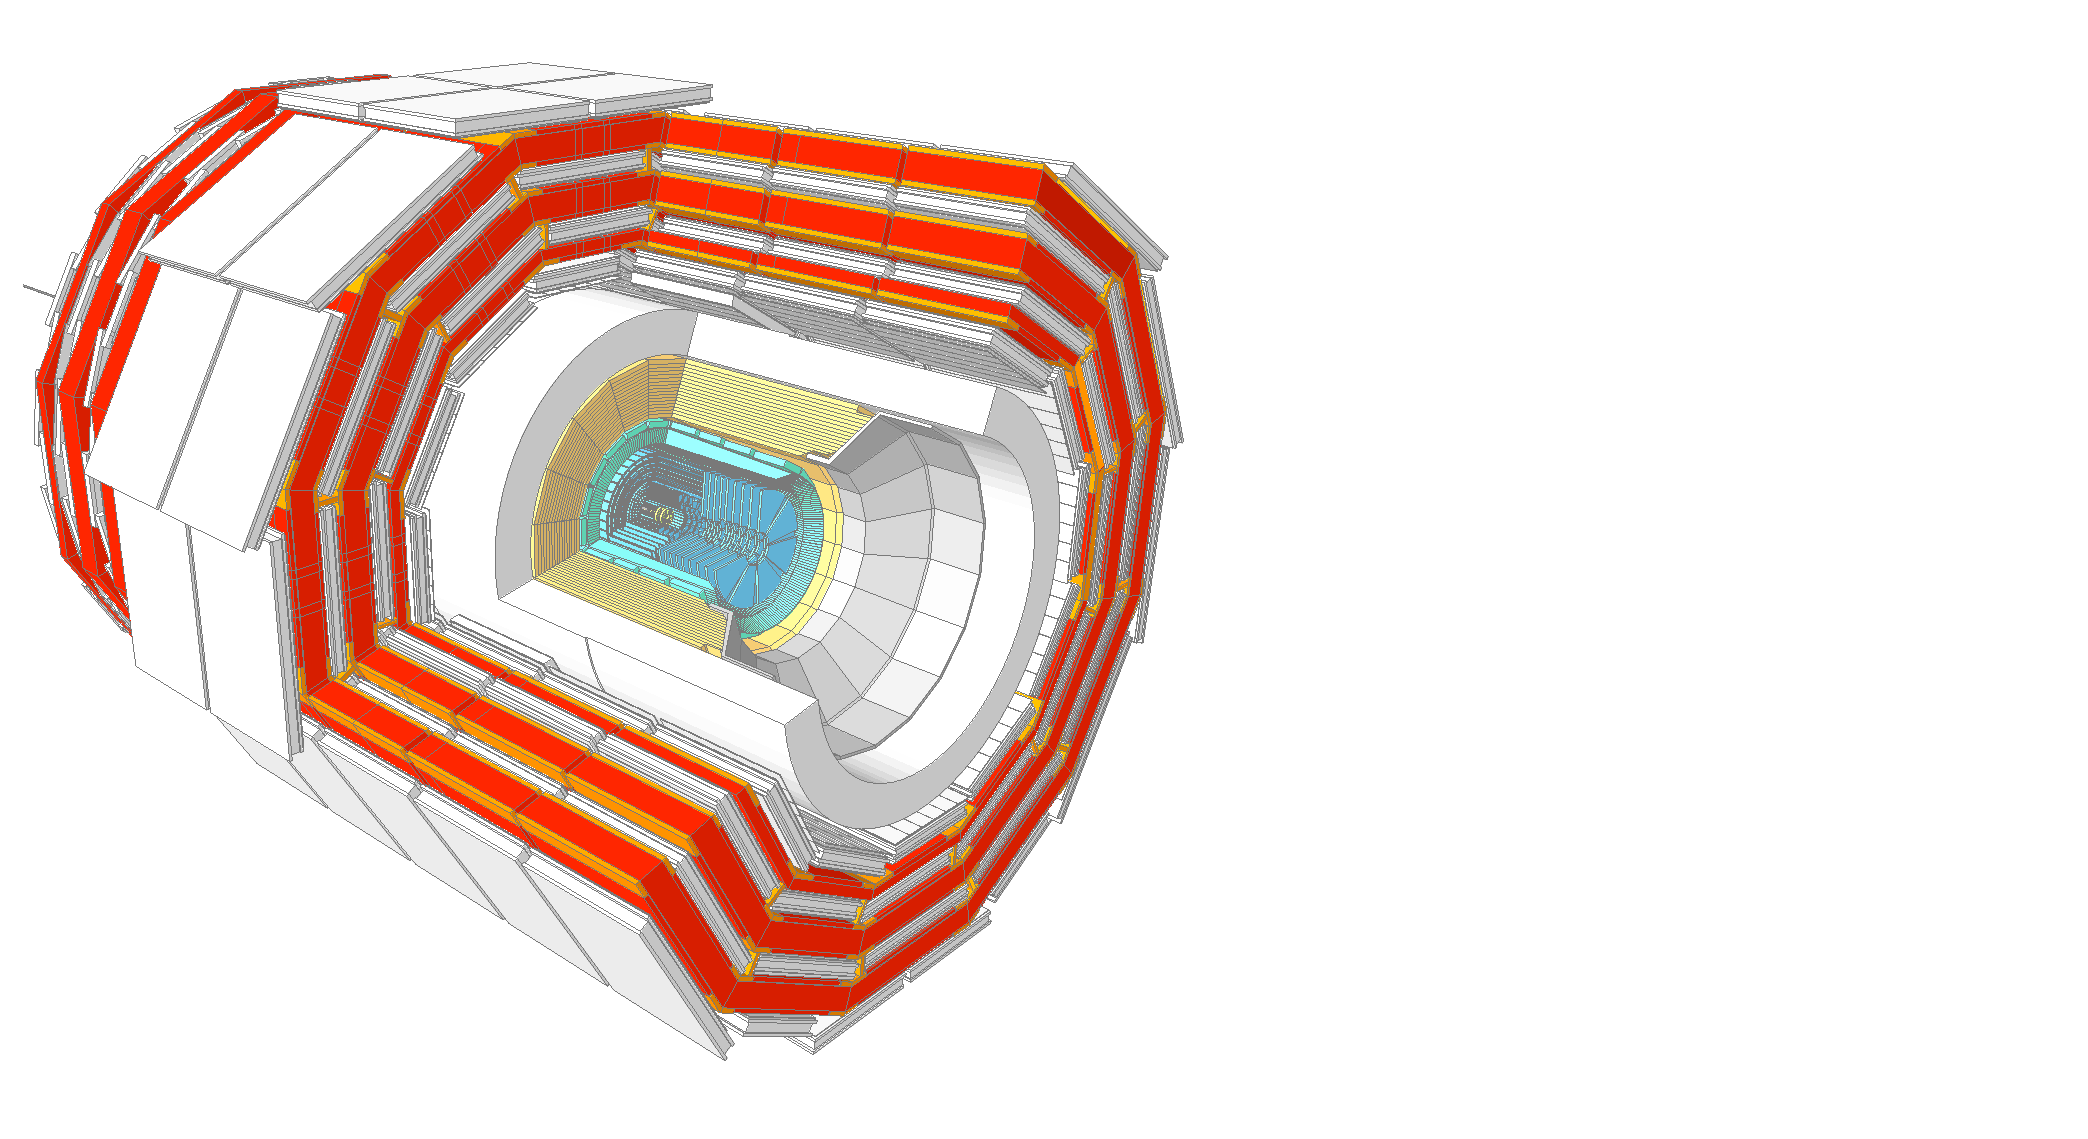
\includegraphics[width=0.9\textwidth]{figures/apparatus/CMS.pdf}
    \begin{center}
        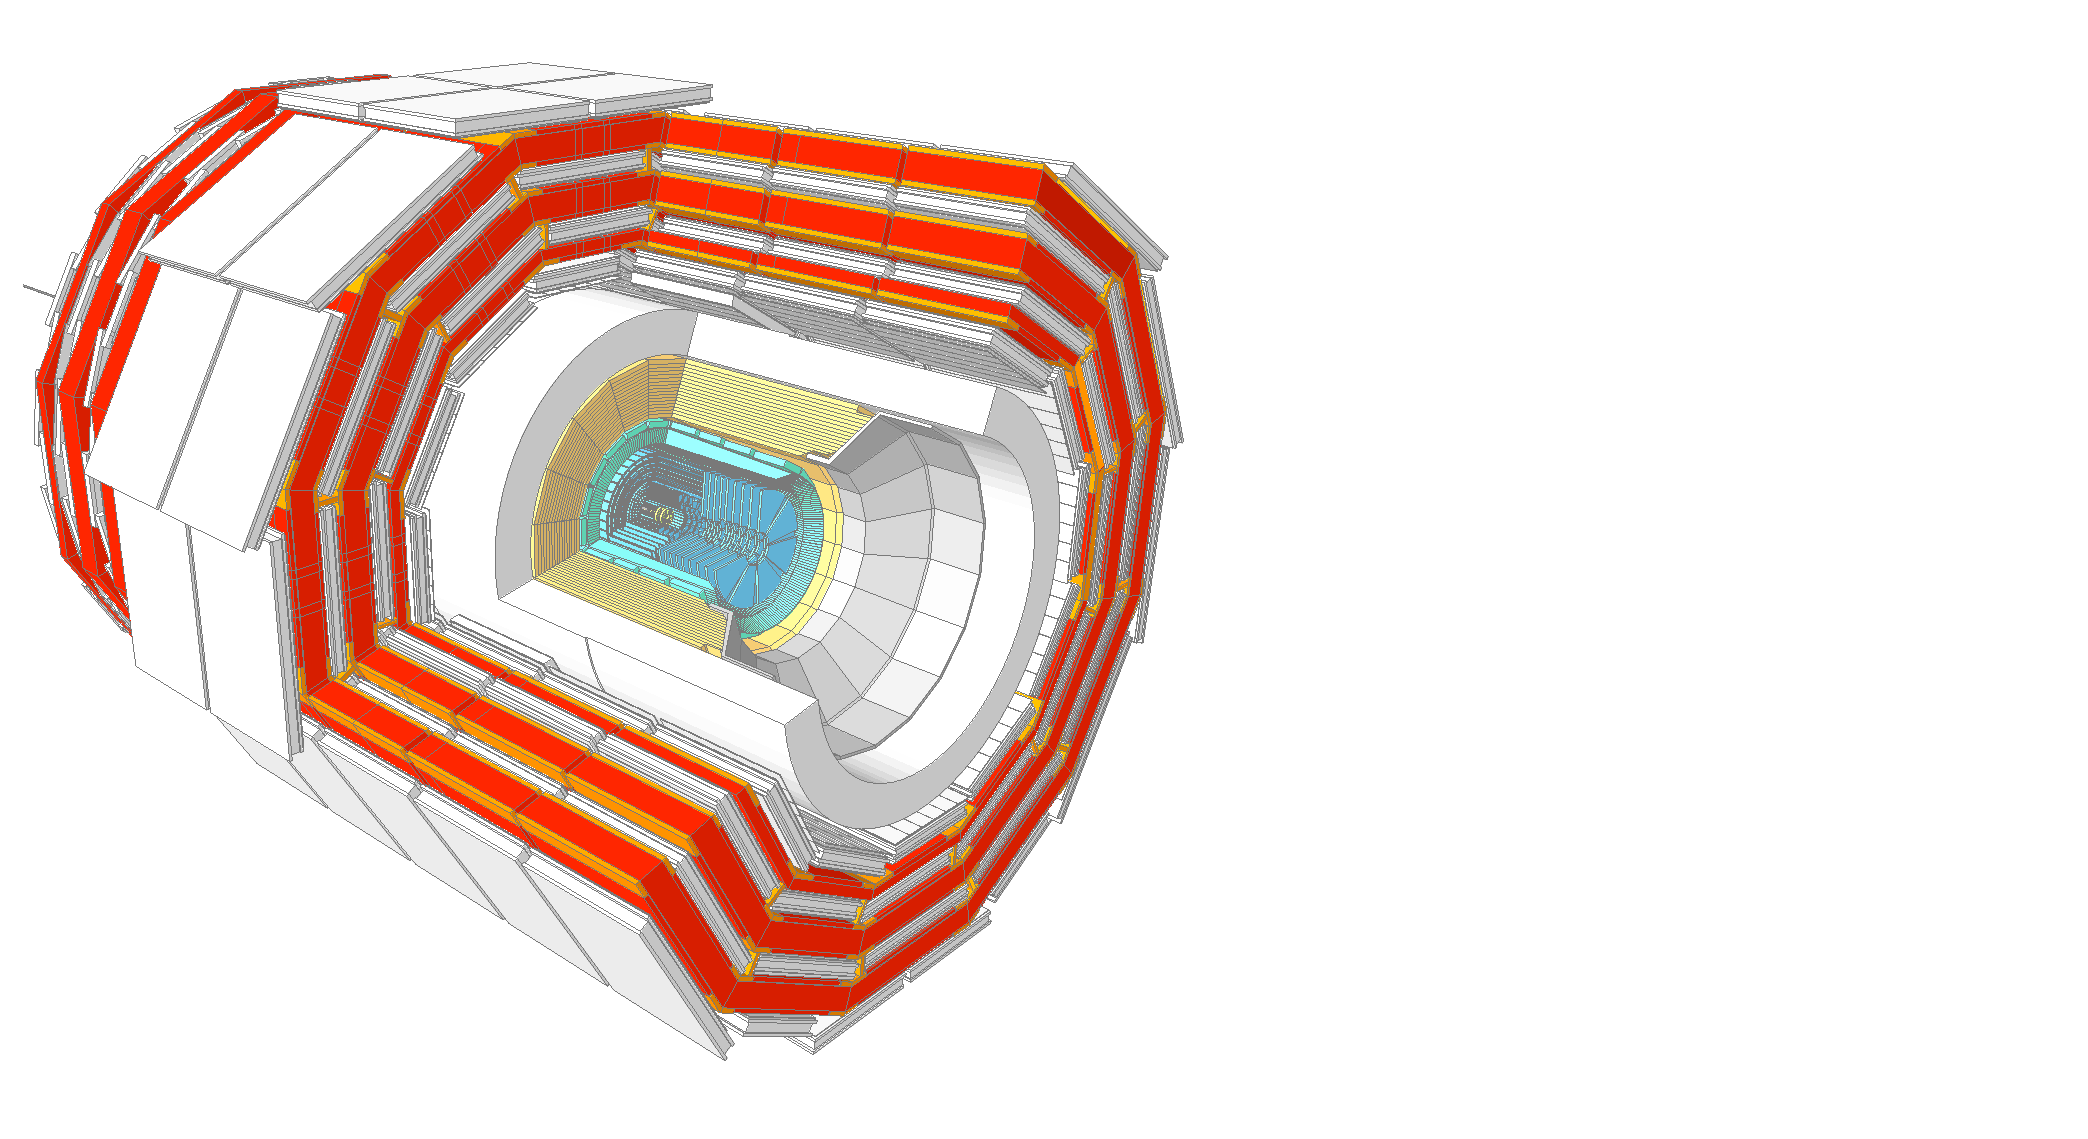
\includegraphics[width=0.57\textwidth]{figures/apparatus/CMS.pdf}
        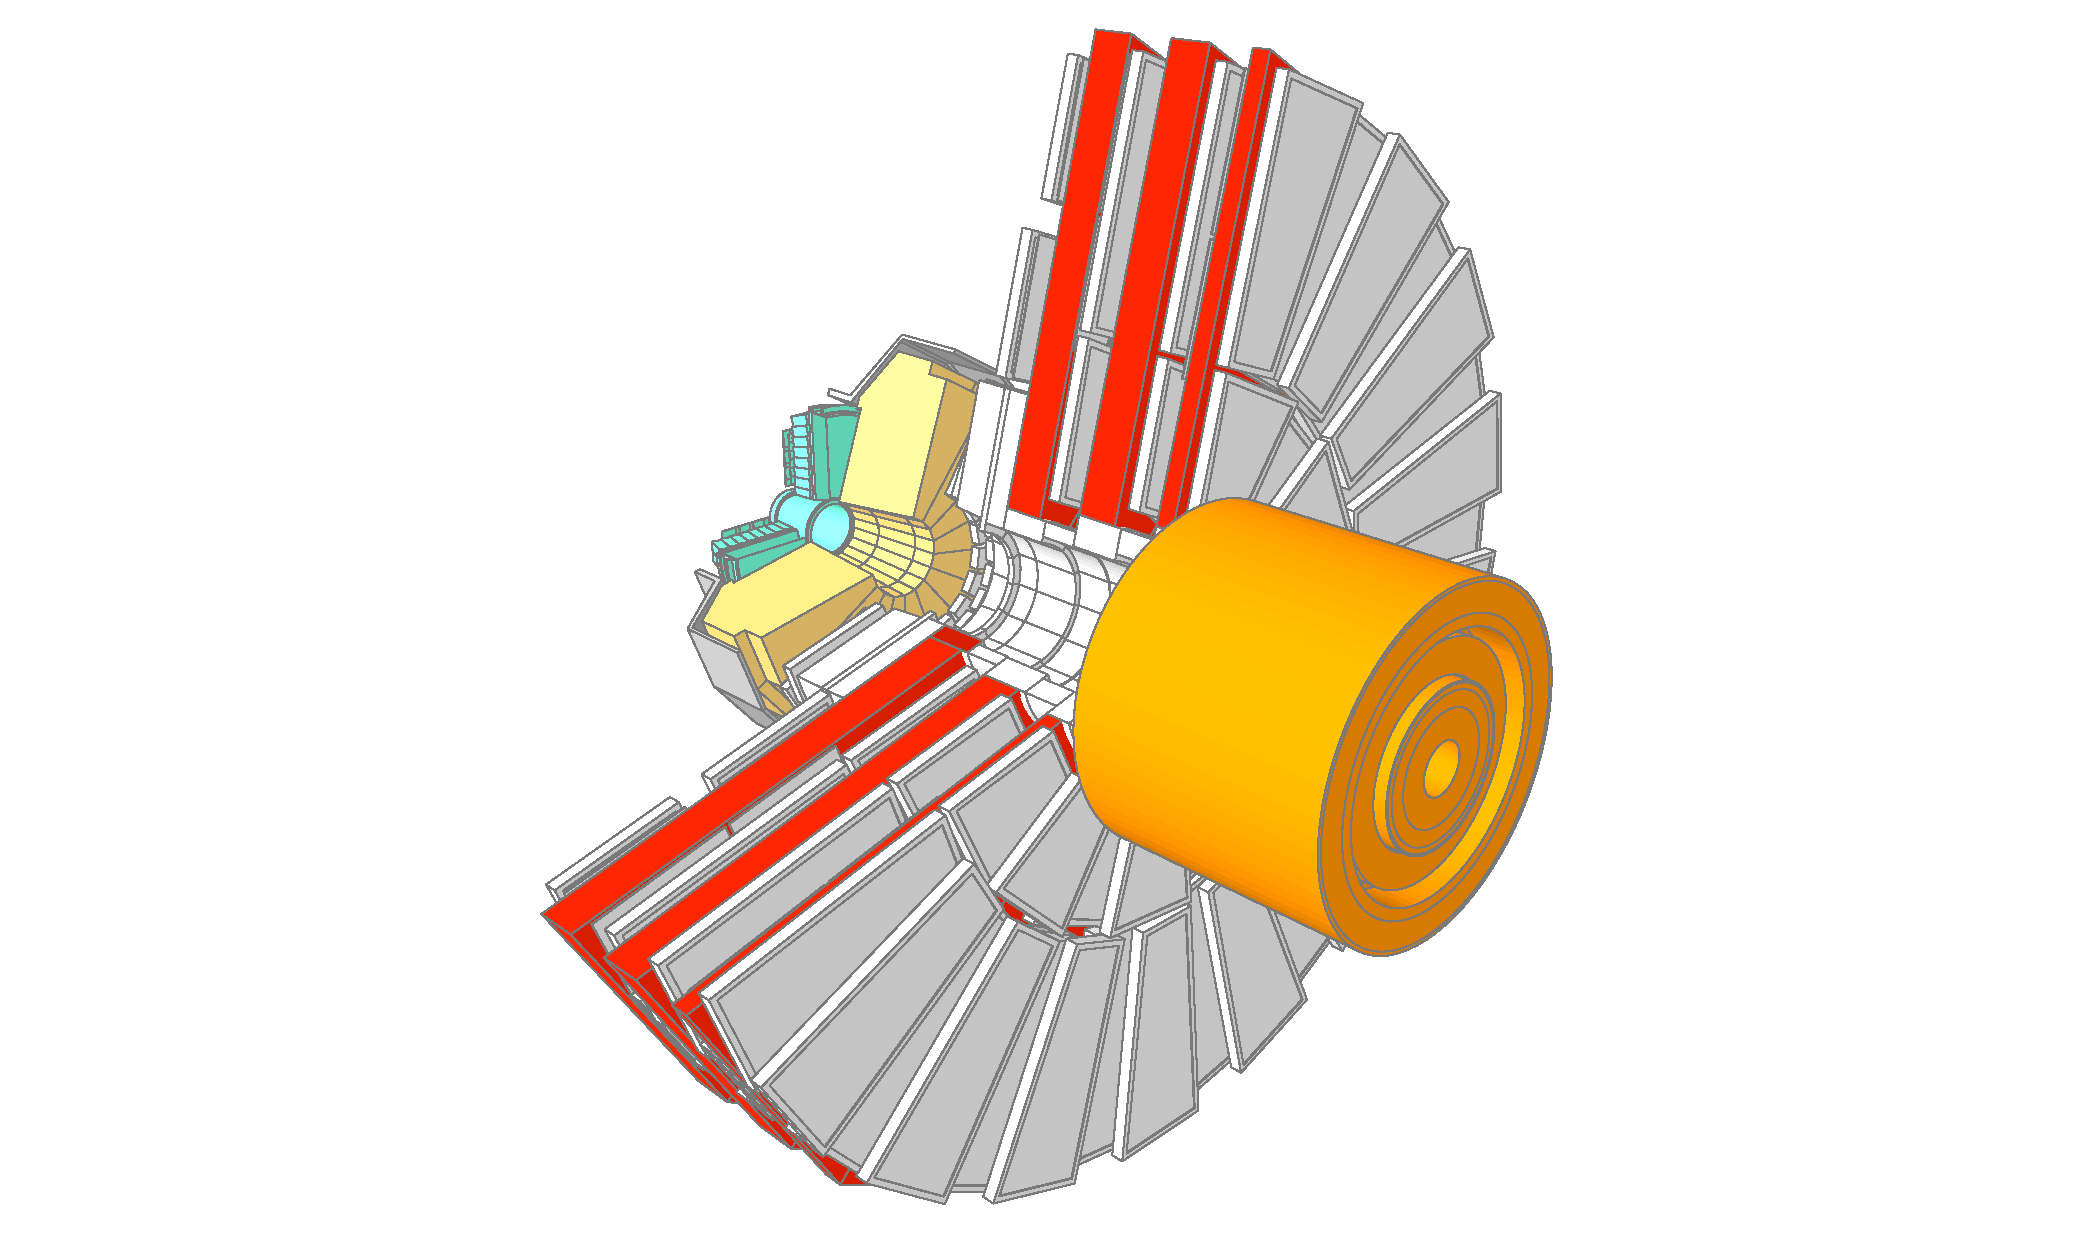
\includegraphics[width=0.42\textwidth]{figures/apparatus/ENDCAP2.pdf}
    \end{center}    
    \caption{The CMS experiment separated into barrel (left) and endcap (right), both have an azimuthal section removed to show structure of the detector subsystems. Rendering was built with the model in \cite{SketchupCMS}.}
    \label{fig:apparatus:CMS}
\end{figure}



The general structure of CMS is a classic hermetic design with a main cylindrical section centred around the interaction point called the `barrel' that is then sealed by two `endcaps' this gives a detector with a pseudorapidity range from $-5$ to $5$ that almost covers the entire $4\pi$ solid angle. Both barrel and endcaps consist of multiple concentric detector subsystems with different functionality, all of this is based around the main feature of the CMS detector: its large superconducting solenoid. 
The CMS solenoid, along with the steel return yoke it is supported by, achieves a high-strength and homogenous magnetic field over a large volume. This field bends the trajectories of charged particles into a helix, and when this bend is measured precisely one can achieve a precise momentum measurement. This meets the performance requirements for momentum resolution of charged particles and especially muons. Within the bore of the solenoid there are three subsystems: the tracker, the electromagnetic calorimeter (ECAL) and the hadron calorimeter (HCAL). The tracker consists entirely of silicon based sensors and performs precise measurements of charged particle trajectories, at the centre are pixel detectors which allow CMS to meet its $\tau$ lepton and $b$-quark jet tagging goals by reconstructing tracks and secondary vertices with great precision. 
After this, the ECAL measures the energy of electromagnetically interacting particles with good resolution. This energy resolution allows for excellent mass resolution for dilepton and diphoton objects and is crucial to the measurement of Higgs boson decays to $\gamma\gamma$ and $ZZ^{(*)}$.
Situated around the ECAL, the HCAL measures the energies of neutral hadrons and covers a large area with fine granularity to achieve hermeticity and to meet the objective of good $E_{T}^{\mathrm{miss}}$ measurement.
Finally, the muon detectors are sited around the outside of the solenoid and cover a large area. These systems are interleaved with the steel return yoke and measure muon trajectories and energy precisely to achieve good muon momentum resolution and particle identification with a fast response. 
Each of these subdetector systems, with the exception of the tracker, provide fast measurements for the CMS trigger system. This allows CMS to cope with the very high data rate by making fast decisions about whether to keep events.
Each of these systems will be described in detail in the following subsections. Particular attention will be given to the ECAL due to its importance to the measurement of the Higgs diphoton decay mode. 


\subsection{Solenoid and Return Yoke}

The CMS magnet is a liquid helium cooled superconducting solenoid 12.5\,m in length with a bore of diameter 6\,m and a mass of 220\,t (including all systems operating at cryogenic temperature) \cite{CMSPhysics}. 
This is situated within a steel return yoke \cite{Yoke} that weighs 12000\,T extends outwards to a diameter of 14\,m and is made of five barrel `wheels' with three layers, and then completed by three disks in each endcap (Figure \ref{fig:apparatus:solenoid_yoke}).
\begin{figure}[h!]
    \centering
    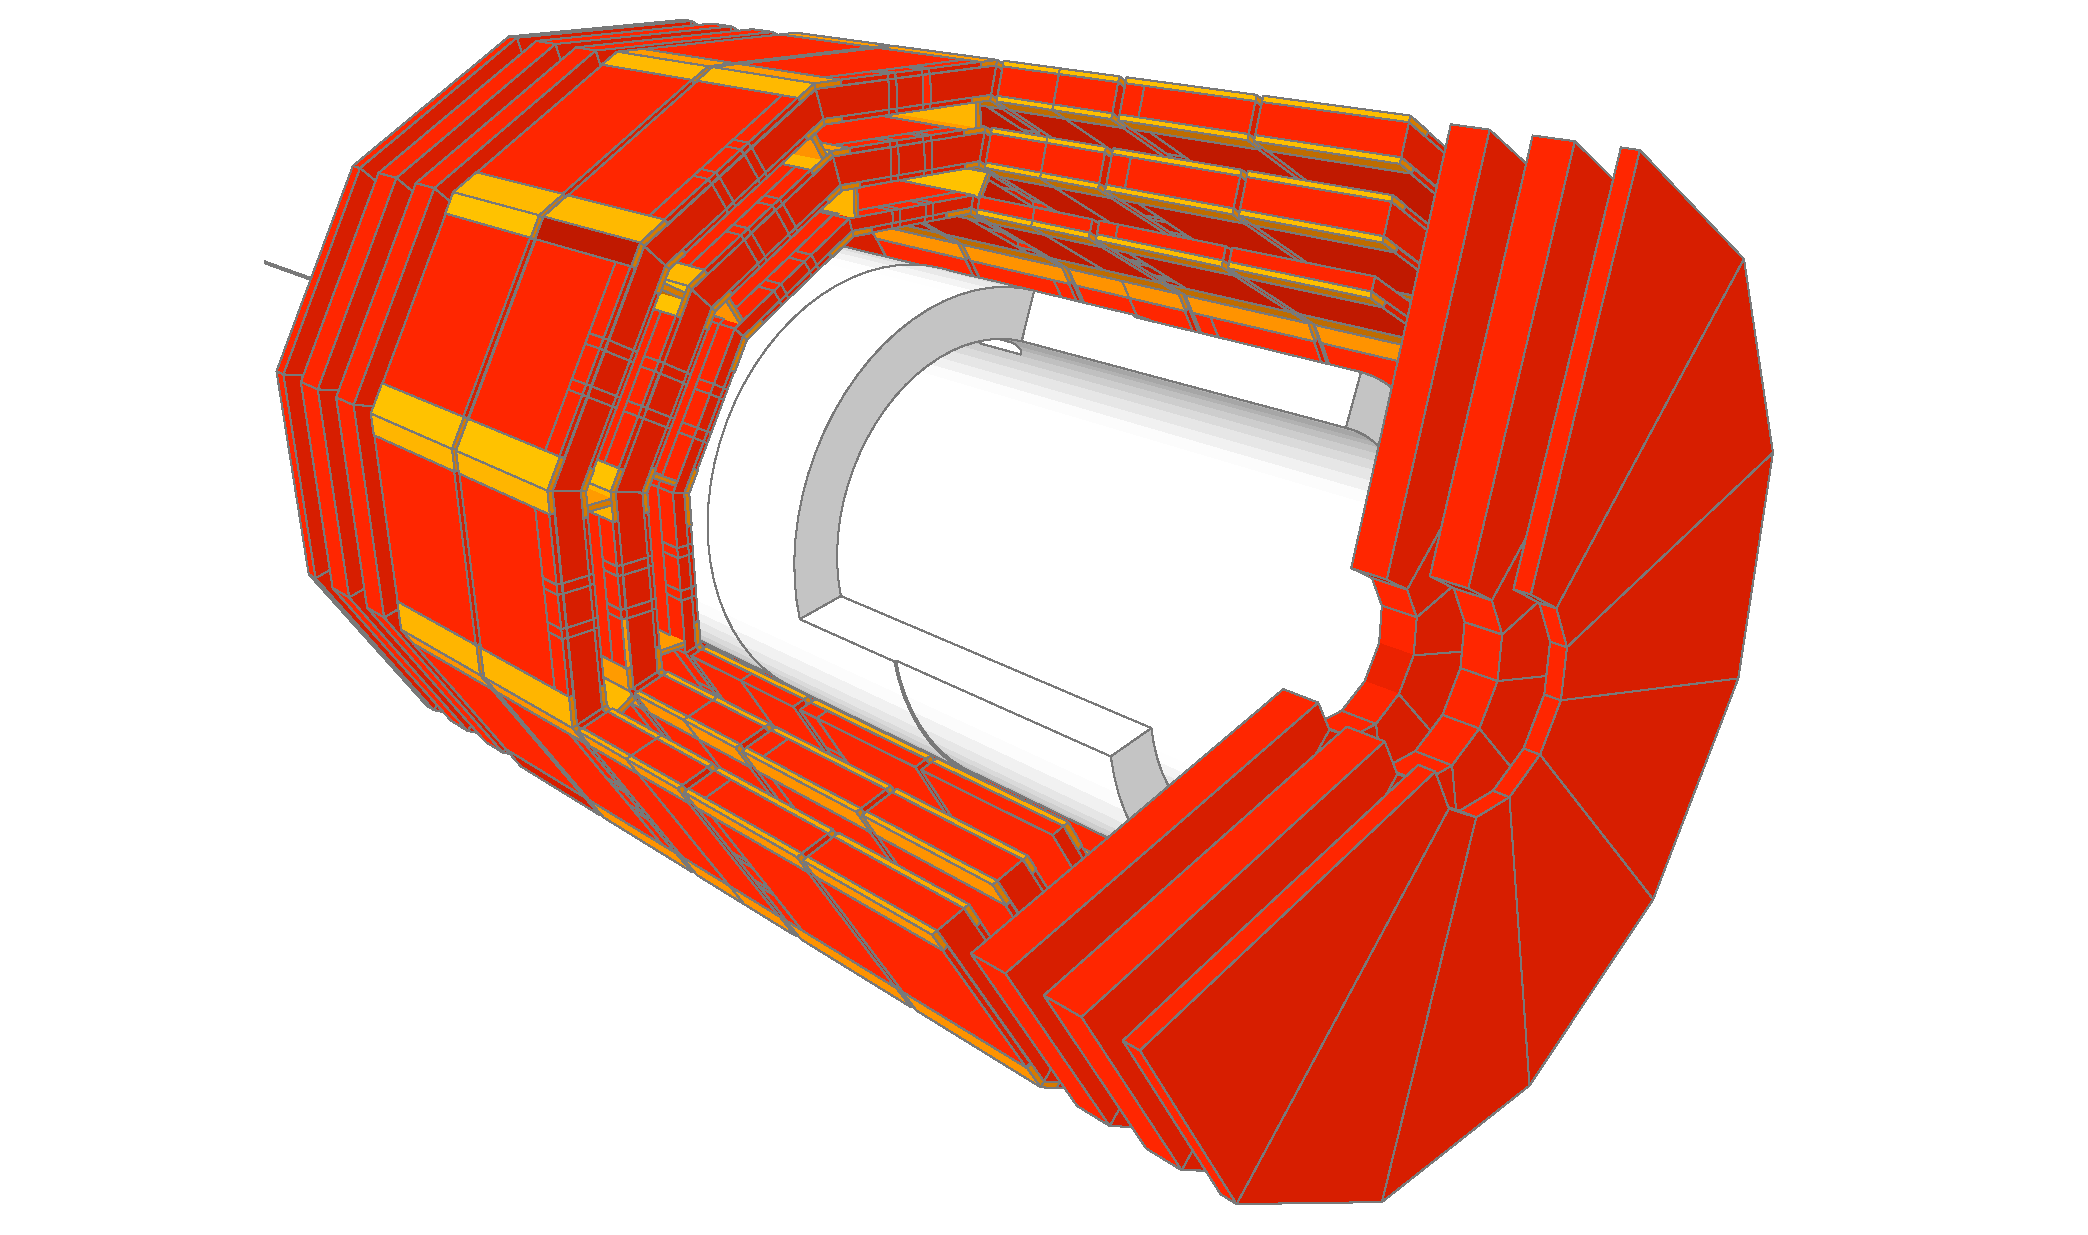
\includegraphics[width=0.5\textwidth]{figures/apparatus/solenoid_yoke.pdf}
    \caption{The CMS solenoid (white) within the steel return yoke (red). Rendering uses \cite{SketchupCMS}.}
    \label{fig:apparatus:solenoid_yoke}
\end{figure}
The niobium-titanium coils of the solenoid carry 18160\,A of current that produces a magnetic field strength within the bore of 3.8\,T and a stored energy of 2.3\,GJ. 
This field strength is below the design capability of 4\,T to maximise the operating lifetime of the solenoid.
The return yoke then conditions this field, increasing the strength in the bore by a small amount (8\%) \cite{Yoke} and improving the field homogeneity in the barrel and the muons systems. 


\subsection{Inner Tracking}

The CMS tracker \cite{CMSTrackerTDR} is the innermost detector layer and is designed to measure the trajectories and the secondary vertices of charged particles with high precision. 
To meet the requirements of the LHC operating environment the tracker must have fine granularity to handle the high-multiplicity environment, precise timing to match the particle tracks to the correct bunch crossing, and it must be robust to large doses of radiation.
It must also introduce minimal material in front of the other detector subsystems to avoid photon conversion, bremsstrahlung and other interactions. This would particularly degrade the quality of reconstructed photons and electrons. 
These requirements motivated the choice of silicon sensor technology for the tracker that uses two different types: pixel detectors and microstrip detectors. Pixel detectors are made up of many small pixels and measure a position on a trajectory in two dimensions, microstrips consist of small parallel strips separated by a distance called the `pitch' that detects the ionisation from an incident charged particle in one dimension. 


The general structure of the tracker (Figure \ref{fig:apparatus:tracker}) has a length of 5.8\,m, a diameter of 2.5\,m and covers a pseudorapidity range of $|\eta|<2.5$. Its active surface consists of 1440 pixel sensors, 15148 microstrip detectors and covers an area of approximately 200\,m$^{2}$. 
\begin{figure}[h!]
    \begin{center}
        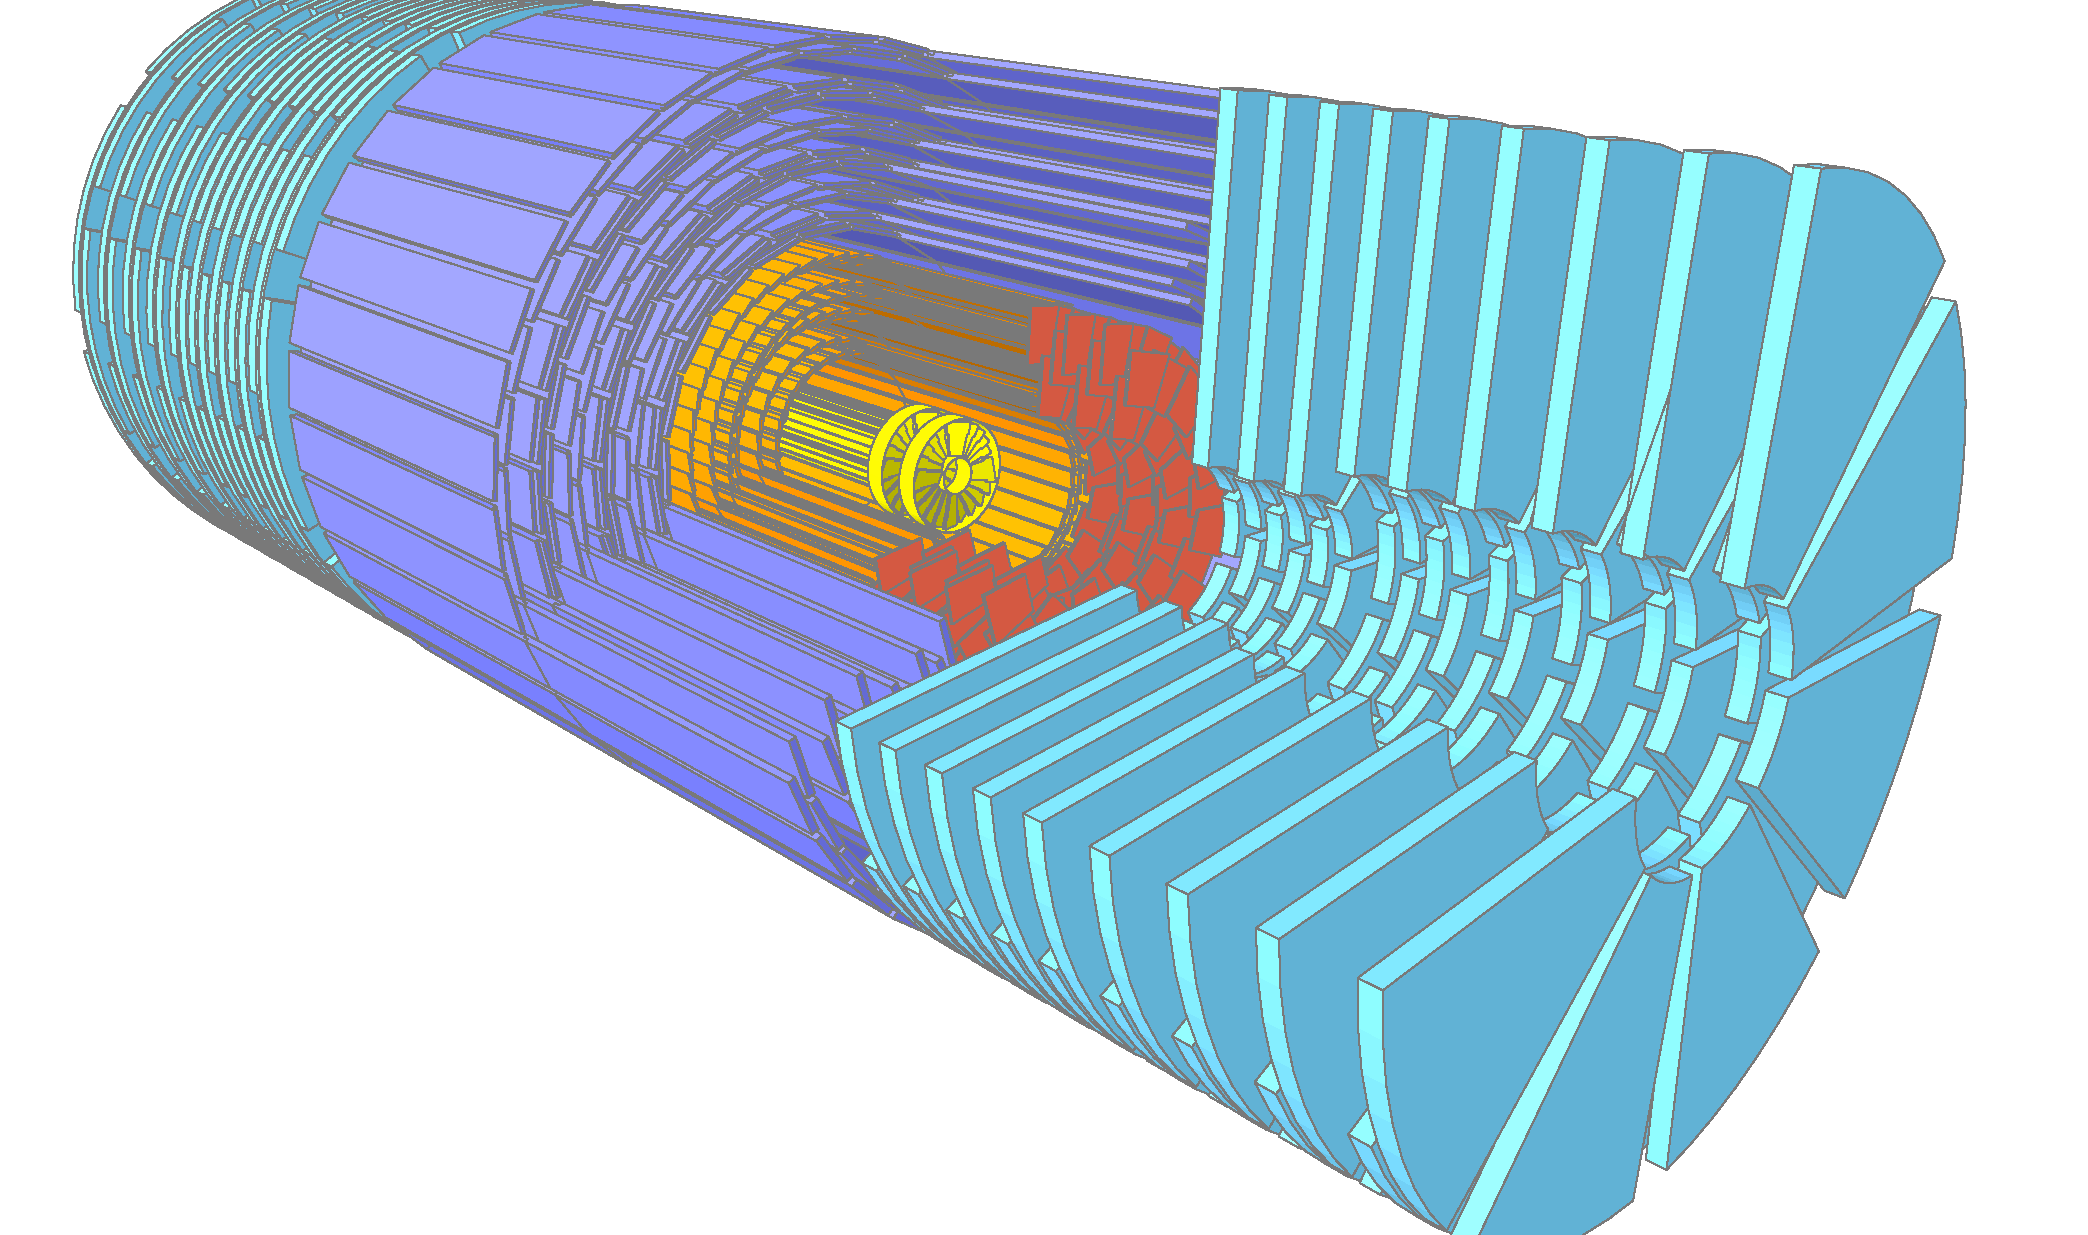
\includegraphics[width=0.6\textwidth]{figures/apparatus/tracker_colour.pdf}
        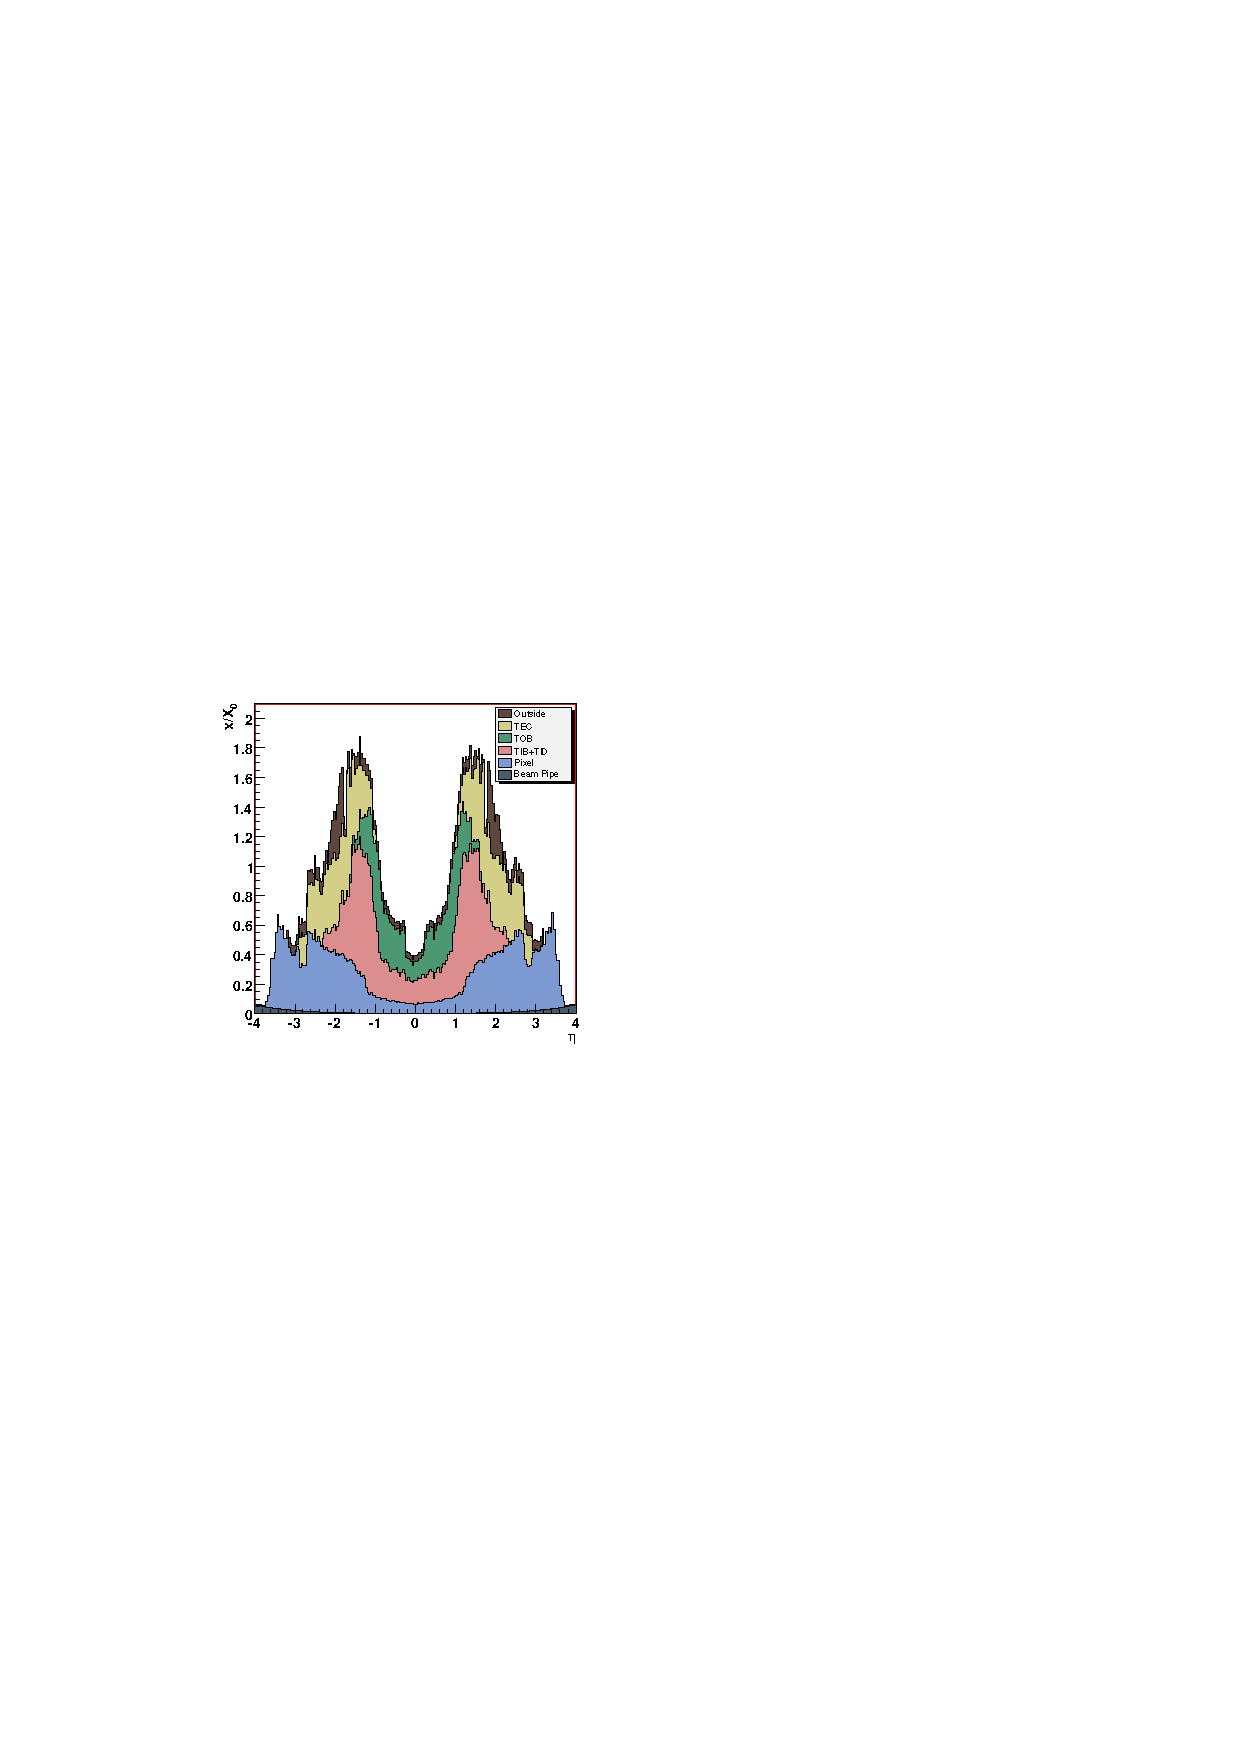
\includegraphics[width=0.39\textwidth]{figures/apparatus/tracker_material.pdf}
    \end{center}
    \caption{Left: the tracker subsystem showing the the central pixel detector in yellow, TIB in orange, TID in red, TOB in purple and TECs in blue \cite{SketchupCMS}. Right: the material before the ECAL in radiation lengths ($X_{0}$) \cite{CMSatLHC}.}
    \label{fig:apparatus:tracker}
\end{figure}
These are assembled into several subsystems: the pixel, the tracker inner barrel (TIB), the tracker inner disks (TID), the tracker outer barrel (TOB) and the tracker endcaps (TEC).

The innermost subsystem of the tracker is the pixel detector which provides precise measurements in $\phi$, $r$ and $z$ of particle trajectories and achieves a high transverse and longitudinal position resolution. The pixel consists of pixel sensors arranged in cylinders of 4.4\,cm, 7.3\,cm, and 10.2\,cm with two disks of pixels sensors at either end to give a total of 66 million pixels and an active area of 1\,m$^{2}$. This gives a pseudorapidity coverage of $|\eta|<2.5$ and at least three position determinations along each track with a transverse resolution of 10\,$\mu$m and longitudinal resolution of 20-40\,$\mu$m. Further out from the pixel detector all of the tracker subsystems use silicon microstrip sensors. 


Situated around the pixel detector are the TIB and TID subsystems that extend in radius out to 55\,cm and consist of four cylinders of sensors in the TIB and three disks of sensors in the TID. These deliver up to four $r$-$\phi$ measurements using sensors oriented parallel to the beam axis in the barrel and radially on the disks. These sensors have a pitch of 80\,$\mu$m in layers one and two of the TIB and 120\,$\mu$m further out giving a position resolution of 23\,$\mu$m and 35\,$\mu$m respectively. 
Surrounding the TIB and TID is the TOB subsystem with an outer radius of 116\,cm, $z$ between $\pm$118\,cm and consists of six cylindrical layers with pitches of 183\,$\mu$m in the first four layers and 122\,$\mu$m in the fifth and sixth. This gives six $r$-$\phi$ measurements with single point resolutions of 53\,$\mu$m and 35\,$\mu$m respectively. 
Finally, at either end, are the TEC tracker subsystems that extend in radius from 22.5\,cm to 113.5\,cm and extend in $|z|$ between 124\,cm and 282\,cm. Each of the two TECs consist of nine disks of up to seven rings of radially-oriented microstrip sensors. This gives up to nine measurements of $\phi$ for each trajectory.  
Some of the microstrip modules are in pairs to provide a second coordinate measurement: $z$ in the cylindrical layers, $r$ in the discs. They are mounted back to back and rotated by 100\,mrad with respect to each other. These modules make up the first two layers of the TIB and TOB, the first two rings of the TID and the first, second and fifth rings of the TECs.  
All of this ensures $\approx$9 precision measurements of trajectories in the silicon microstrip part of the tracker in the range $|\eta|<2.4$ with $\approx$4 of them being two-dimensional.


The entire tracker material budget manages to remain under two radiation lengths: it ranges from $0.4$\,$X_{0}$ at $|\eta|\approx{0}$ to about $1.8$\,$X_{0}$ at $|\eta|\approx{1.4}$ back to about $1$\,$X_{0}$ at $|\eta|\approx{2.5}$. This is shown in Figure \ref{fig:apparatus:tracker}.


\subsection{Electromagnetic Calorimetry}

The CMS ECAL \cite{CMSEcalTDR} is a calorimeter designed to reconstruct the energy of electromagnetically interacting particles such as photons with good resolution. In particular the ECAL is aimed at the detection and reconstruction of leptonic and diphoton Higgs final states with good mass resolution within the confines of the CMS solenoid and in LHC operating conditions. To meet these requirements the ECAL must have fine spatial granularity, a large spatial acceptance, a fast response time, and it must capture maximal information from the showers in the restricted space available within the solenoid. 

%\subsubsection{Geometry}
%Overall geometry
The ECAL as a whole has the following geometry (Figure \ref{fig:apparatus:ecal}): the barrel region (EB) covers a pseudorapidity range of $|\eta|<1.442$, there is then a gap between $1.4442<|\eta|<1.566$, and finally the endcaps (EE) cover the range $1.566<|\eta|<3$. Due to prohibitive radiation and pileup conditions electrons and photons are only measured with precision up to $|\eta|<2.5$. 
In addition to these subsystems there is the preshower detector (ES) mounted in front of the endcaps that occupies the range $1.54<|\eta|<2.61$. The ES consist of two disks of lead absorber followed by two planes of silicon strip detectors with pitch $1.9$\,mm. This is used for $\pi_{0}$ rejection. 
\begin{figure}[h!]
    \centering
    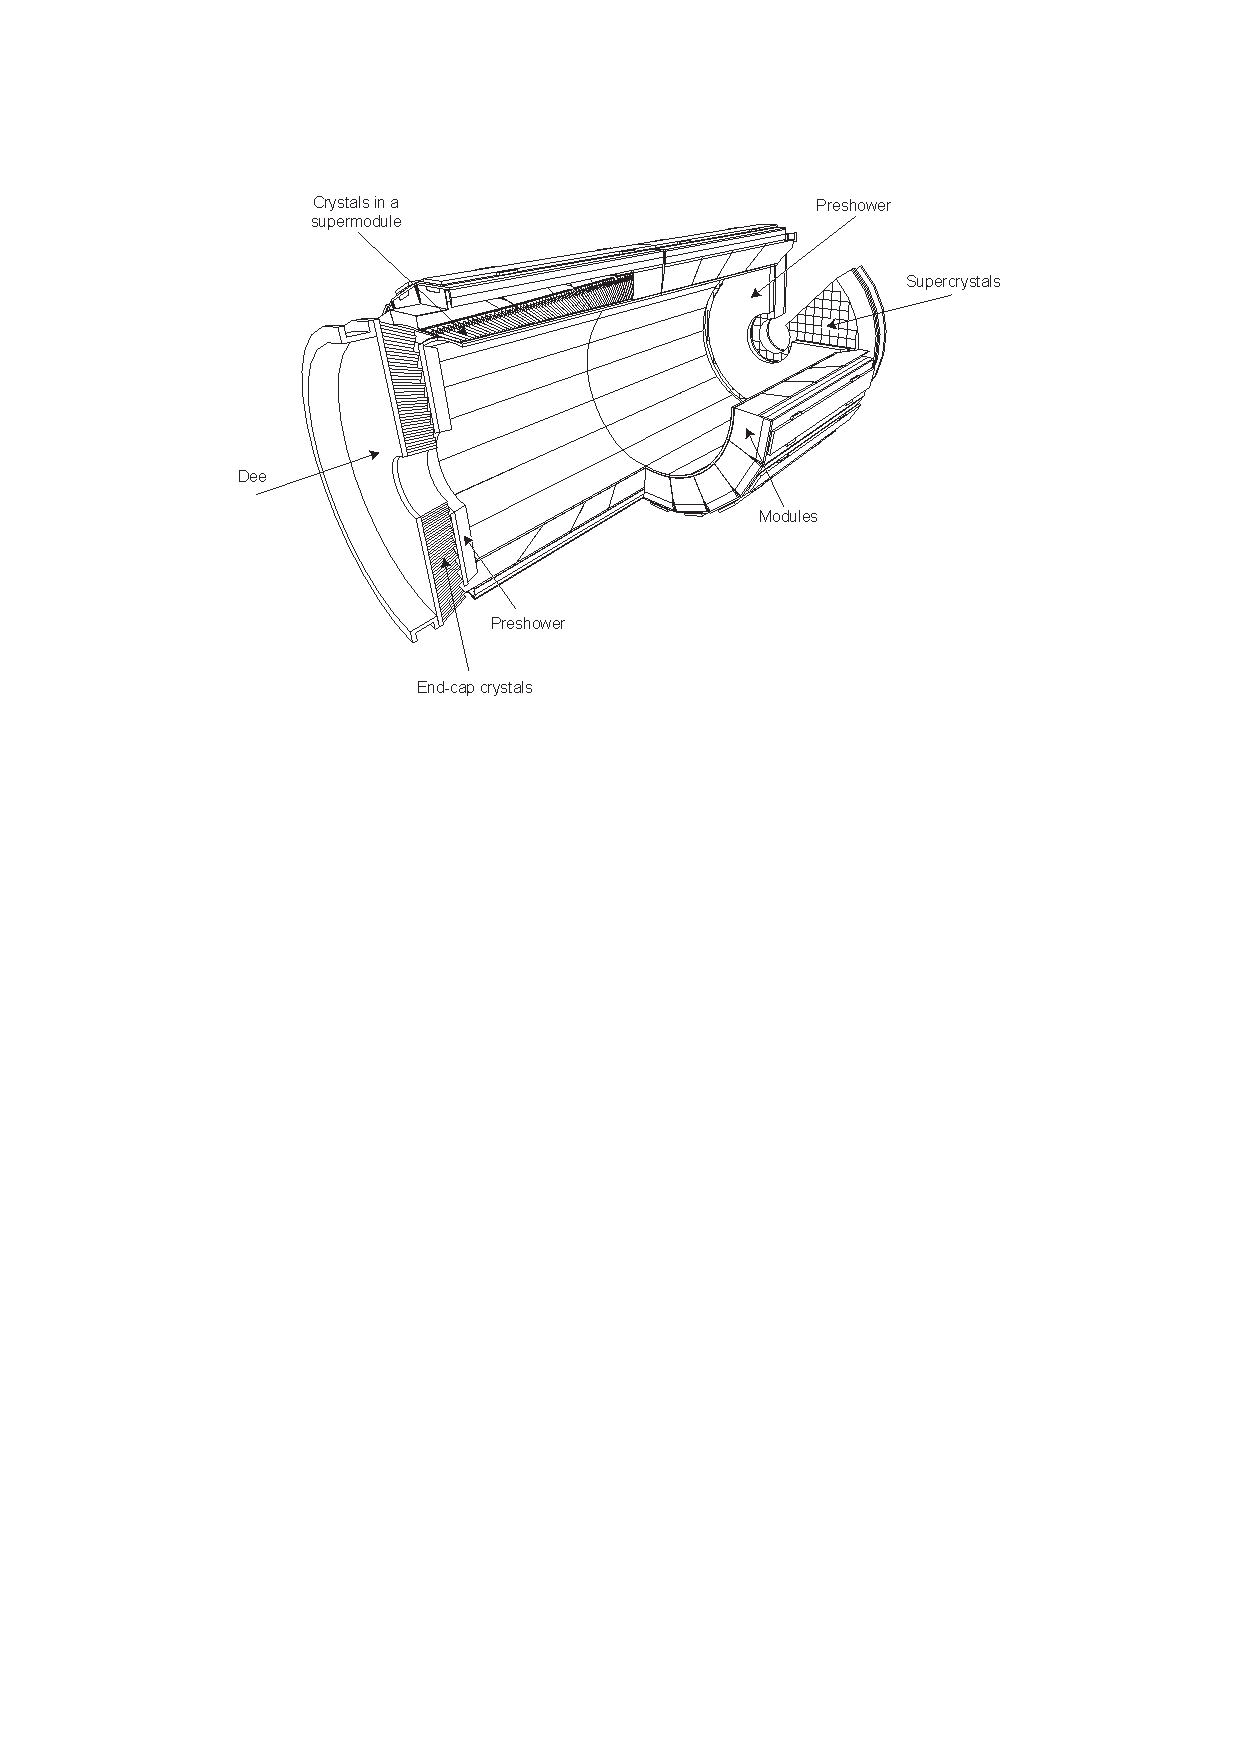
\includegraphics[width=0.9\textwidth]{figures/apparatus/ECAL_alt.pdf}
    \caption{The CMS ECAL with a section removed to show structure \cite{CMSatLHC}.}
    \label{fig:apparatus:ecal}
\end{figure}

%Crystal geometry
The EB and the EE regions are constructed out of lead tungstate (PbWO$_{4}$) crystals, 61200 in the former and 7324 in the latter. The choice of PbWO$_{4}$ was made due to its short radiation length (0.89\,cm), and small Moli\`{e}re radius. The short radiation length ensures that particle showers are shorter in extent and can be contained in as small a depth as possible. The short Moli\`{e}re radius (a measure of showers spread transverse to their direction in a material) ensures that the showers are more contained in the $\eta$,$\phi$ directions. 

%Barrel
In the EB each crystal has a front face of 22x22\,mm$^{2}$ corresponding to the Moli\`{e}re radius of 21.9\,mm and a segmentation of $(\Delta\eta,\Delta\phi) = (0.0174,0.0174)$. 
The crystals are also tapered in $\eta$ with 25.8\,$X_{0}$ length (230\,mm) and are oriented at a $3^{\circ}$ offset from the average primary vertex position in $\eta$ and $\phi$. This improves the hermeticity.
%Endcap
In the EE the crystals have a front face of $28.6\times{}28.6$\,mm, are 24.7\,$X_{0}$ (220\,mm) in length. 

%Crystal groupings
The individual crystals are grouped together in both the EB and EE. In the EB they are grouped into 36 `supermodules' that cover a $\Delta\phi = 20^{\circ}$ and extend half the barrel length in $z$.
In each EE identically-shaped crystals are grouped into $5\times5$ `supercrystals' arranged in a rectangular $x$-$y$ grid with angular offsets of $2$-$8^{\circ}$.

%\subsubsection{Electronics and trigger}
When a particle enters one of the crystals and then showers scintillation light will be produced and collected by a sensor at the opposite end. This sensor will produce a pulse that is amplified and then converted into a digital signal. The height of this digitised pulse is then used to determine the energy deposition within the crystal. 
Two different types of sensor are used: in the barrel region avalanche photodiodes are used, the endcaps vacuum phototriodes are used due to the different magnetic field properties and higher radiation levels.
Crystals are read out as $5\times{5}$ trigger towers whose digital signal sum constitutes the fast, coarse information provided to the trigger system with every bunch crossing.


%\subsubsection{Calibration and performance}

The energy resolution of a single PbWO$_{4}$ crystal is modelled with the following equation \cite{CMSPhysics}
\begin{equation}
    \label{eq:apparatus:ecal_energy_reso}
        \left( \frac{\sigma}{E} \right)^{2} =  
        \left( \frac{S}{\sqrt{E}} \right)^{2} +  
        \left( \frac{N}{E} \right)^{2} +  
        C^{2},
\end{equation}
where $S$ is the stochastic term, $N$ is a noise term, and $C$ is a constant term. The crystal performance was measured in a test beam and the above parameters determined by fitting a Gaussian function to the reconstructed energy distributions. Their values were measured to be $S=2.8$\,GeV$^{\frac{1}{2}}$, $N=0.12$\,GeV, and $C=0.3$\%.

To reconstruct the energy of a photon or electron, multiple crystals are typically used as the shower spreads in the ECAL, or even starts before it reaches it. 
Clustering algorithms \cite{ecalShower} are used to reconstruct energy from these crystals and assemble them into a supercluster (SC). The energy associated to the supercluster is then calculated as
\begin{equation}
    E_{SC} = F_{SC}G\sum^{N_{c}}_{i=0}A_{i}C_{i}S_{i}(t)
\end{equation}
where $N_{c}$ is the number of crystals in the SC, $A_{i}$ is the amplitude of the pulse of crystal $i$, $S_{i}(t)$ corrects crystal transparency loss due to radiation, $C_{i}$ is a factor that adjusts the response of the crystal, $G$ is a conversion factor from the digital signal to GeV (global energy scale) and $F_{SC}$ is a correction to the SC energy sum due to second order effects.

To calibrate the ECAL \cite{cmsEcalCalibration} one must use a variety of measurements to determine the factors $G$, $C_{i}$, and $S_{i}(t)$ corresponding to calibration of the overall energy scale, uniformity of measurement in space and uniformity over time respectively. 
Corrections over time due to radiation-induced transparency change in the crystals ($S_{i}(t)$) are derived by injecting laser light at 440\,nm every 40 minutes. 

Several methods are used to derive the factors for an even crystal response over the ECAL spatial extent using the symmetries of CMS. Firstly one uses $\phi$ symmetry to find factors in rings of $\eta$ that should all have the same response. 
Other methods reconstruct particles of known mass decaying to diphotons and use this as a standard candle. The mass should be the same in each part of the detector which allows for the determination of regional differences in response. These different methods are combined to give a collection of per-crystal corrections. 

The final factor, the global energy scale, is derived by reconstructing Z bosons decaying to an $e^{+}e^{-}$ pair and comparing the measured dielectron mass to the known Z boson value.














\subsection{Hadron Calorimetry}
The CMS HCAL \cite{cmsHcal} is situated around the ECAL and its function is to identify neutral hadrons, measure their energies and positions, and to determine $E_{T}^{\mathrm{miss}}$ at good resolution over a large acceptance.
It is a sampling calorimeter that uses material to produce particle showers (absorber) distinct from the active material measuring deposited energy, unlike the ECAL which is a homogeneous calorimeter where one material (lead tungstate) performs both functions. 

The structure of the HCAL is shown in Figure \ref{fig:apparatus:hcal}. It consists of a barrel region (HB), two endcaps (HE), a region outside the solenoid (HO), and two forward calorimeters (HF) that take the HCAL acceptance up to $|\eta|<5$. 
\begin{figure}[h!]
    \centering
    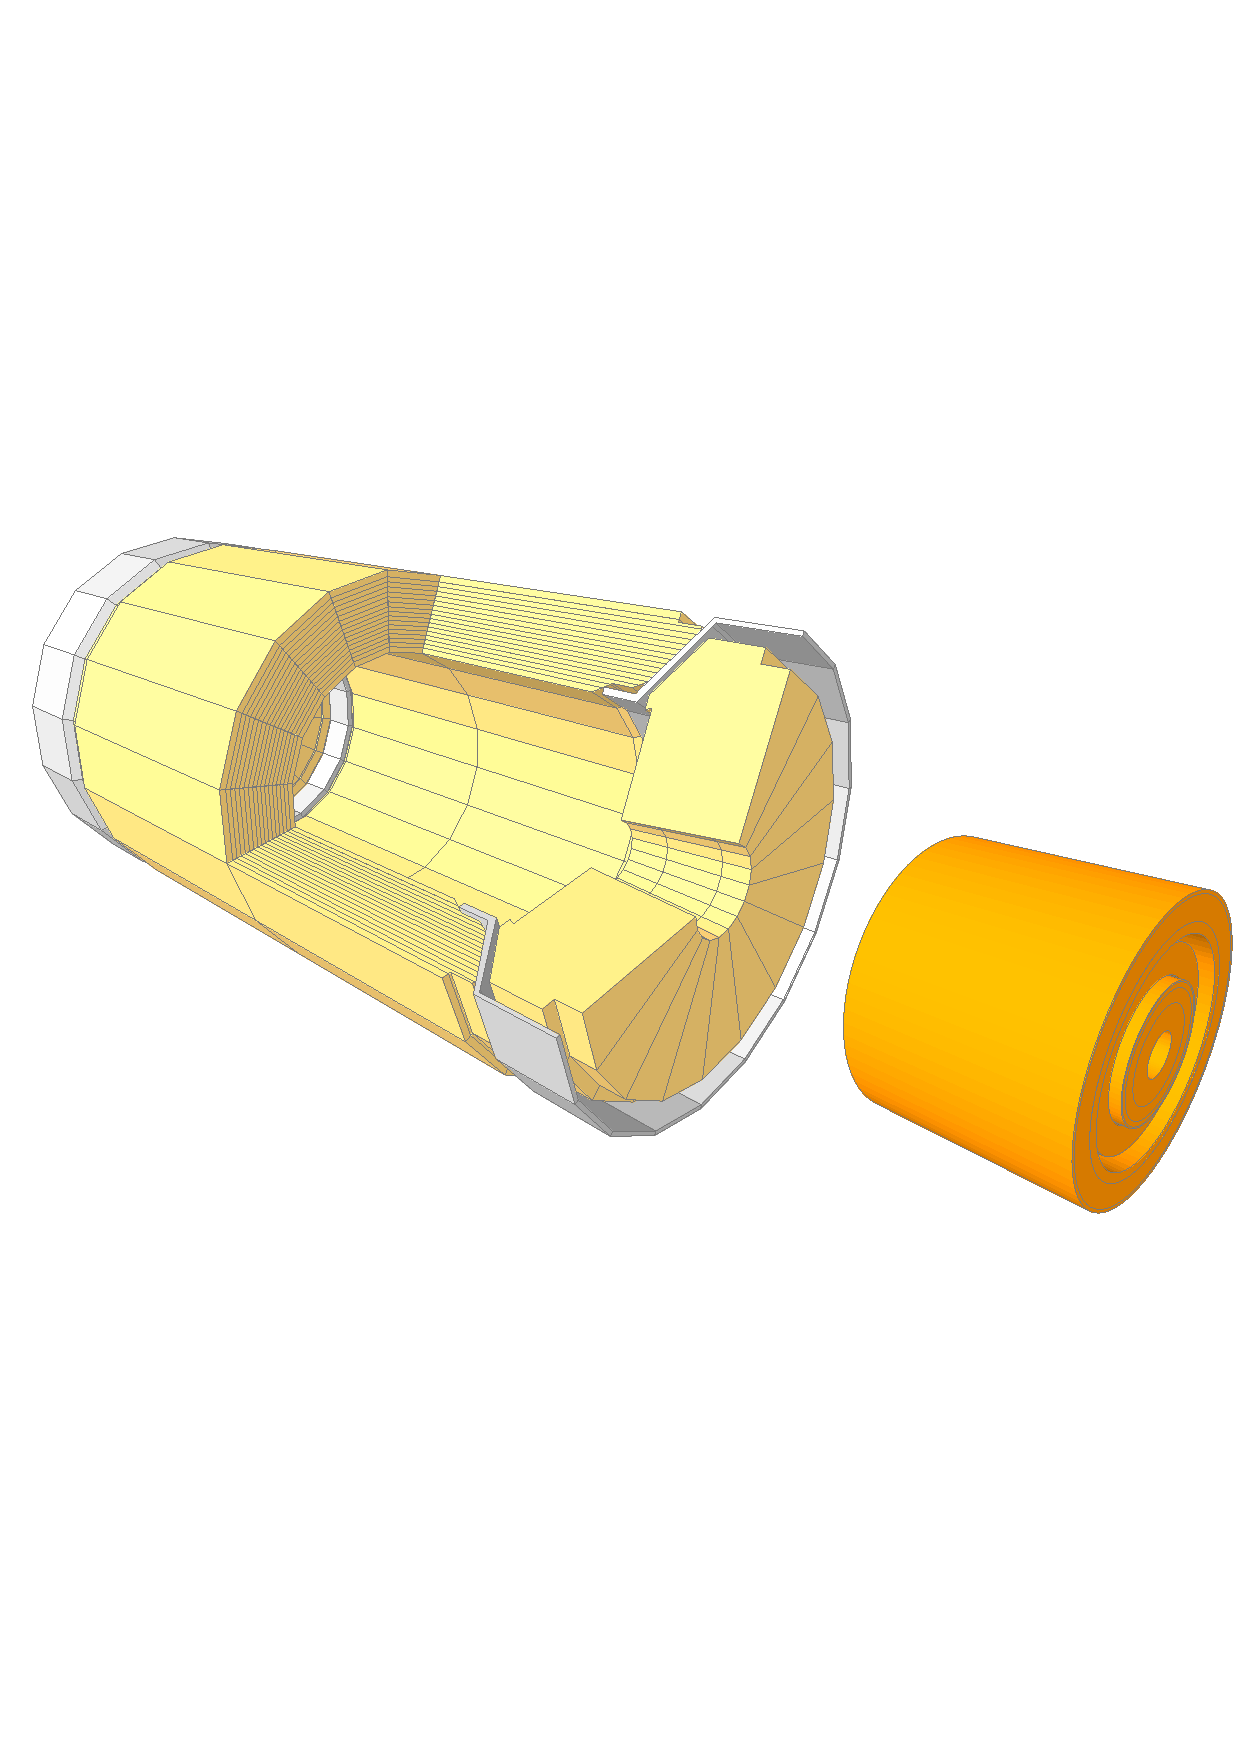
\includegraphics[width=0.8\textwidth]{figures/apparatus/HCAL_HF.pdf}
    \caption{The CMS HCAL with the barrel and endcap sections (left) with part removed to show structure and the forward hadronic calorimeter (right) \cite{SketchupCMS}.}
    \label{fig:apparatus:hcal}
\end{figure}
The HB region covers a pseudorapidity range of $|\eta|<1.3$ and consists of two half-barrel sections that slot in to either end of the solenoid bore that each consist of 36 identical wedges in the azimuthal angle $\phi$. These wedges are constructed from 2 steel and 14 brass absorber plates with a plastic scintillator active material in alternating layers. Brass is used because it is non-magnetic, steel absorber is only used in the innermost and outermost plates to provide structural support. Each wedge is segmented into four azimuthal regions and the plastic scintillator is divided into 16 pseudorapididty regions giving a granularity of $(\Delta\eta,\Delta\phi) = (0.087,0.087)$.
The HE regions cover a pseudorapidity range $1.3<|\eta|<3$ and is divided into 36 azimuthal wedges. It uses brass absorber plates and achieves a granularity between $(\Delta\eta,\Delta\phi) = (0.087,0.087)$ and $(0.017,0.017)$
The HF region covers a pseudorapidity range from $3<|\eta|<5$ and must deal with extremely high levels of radiation. This motivates a different construction with quartz fibres chosen for the active material and steel for the absorber. It is cylindrical in structure with 5\,mm thick grooved plates where the fibres fit into the grooves and operate by detecting Cherenkov light produced by incident particles. The fibres are bundled to form $(\Delta\eta,\Delta\phi) = (0.175,0.175)$ towers.
Finally, the HO covers the barrel region around the solenoid and consists of plastic scintillator tiles matching the granularity of the HB. It uses the solenoid itself as the absorber and is designed to operate as a shower `tail catcher' that compensates for hadron showers that begin later in the HCAL and may not be properly measured. This leakage has a direct effect on the measurement of $E_{T}^{\mathrm{miss}}$.



\subsection{Muon Detection}

The CMS muon system \cite{cmsMuon} is situated around the outside of the solenoid and consists of detectors interleaved with the steel return yoke assembled into barrel and endcap regions (Figure \ref{fig:apparatus:muon}).
The muon system has three objectives: to identify muons, to measure their momentum with precision, and to trigger on them over a large spatial acceptance. 
\begin{figure}[h!]
    \begin{center}
        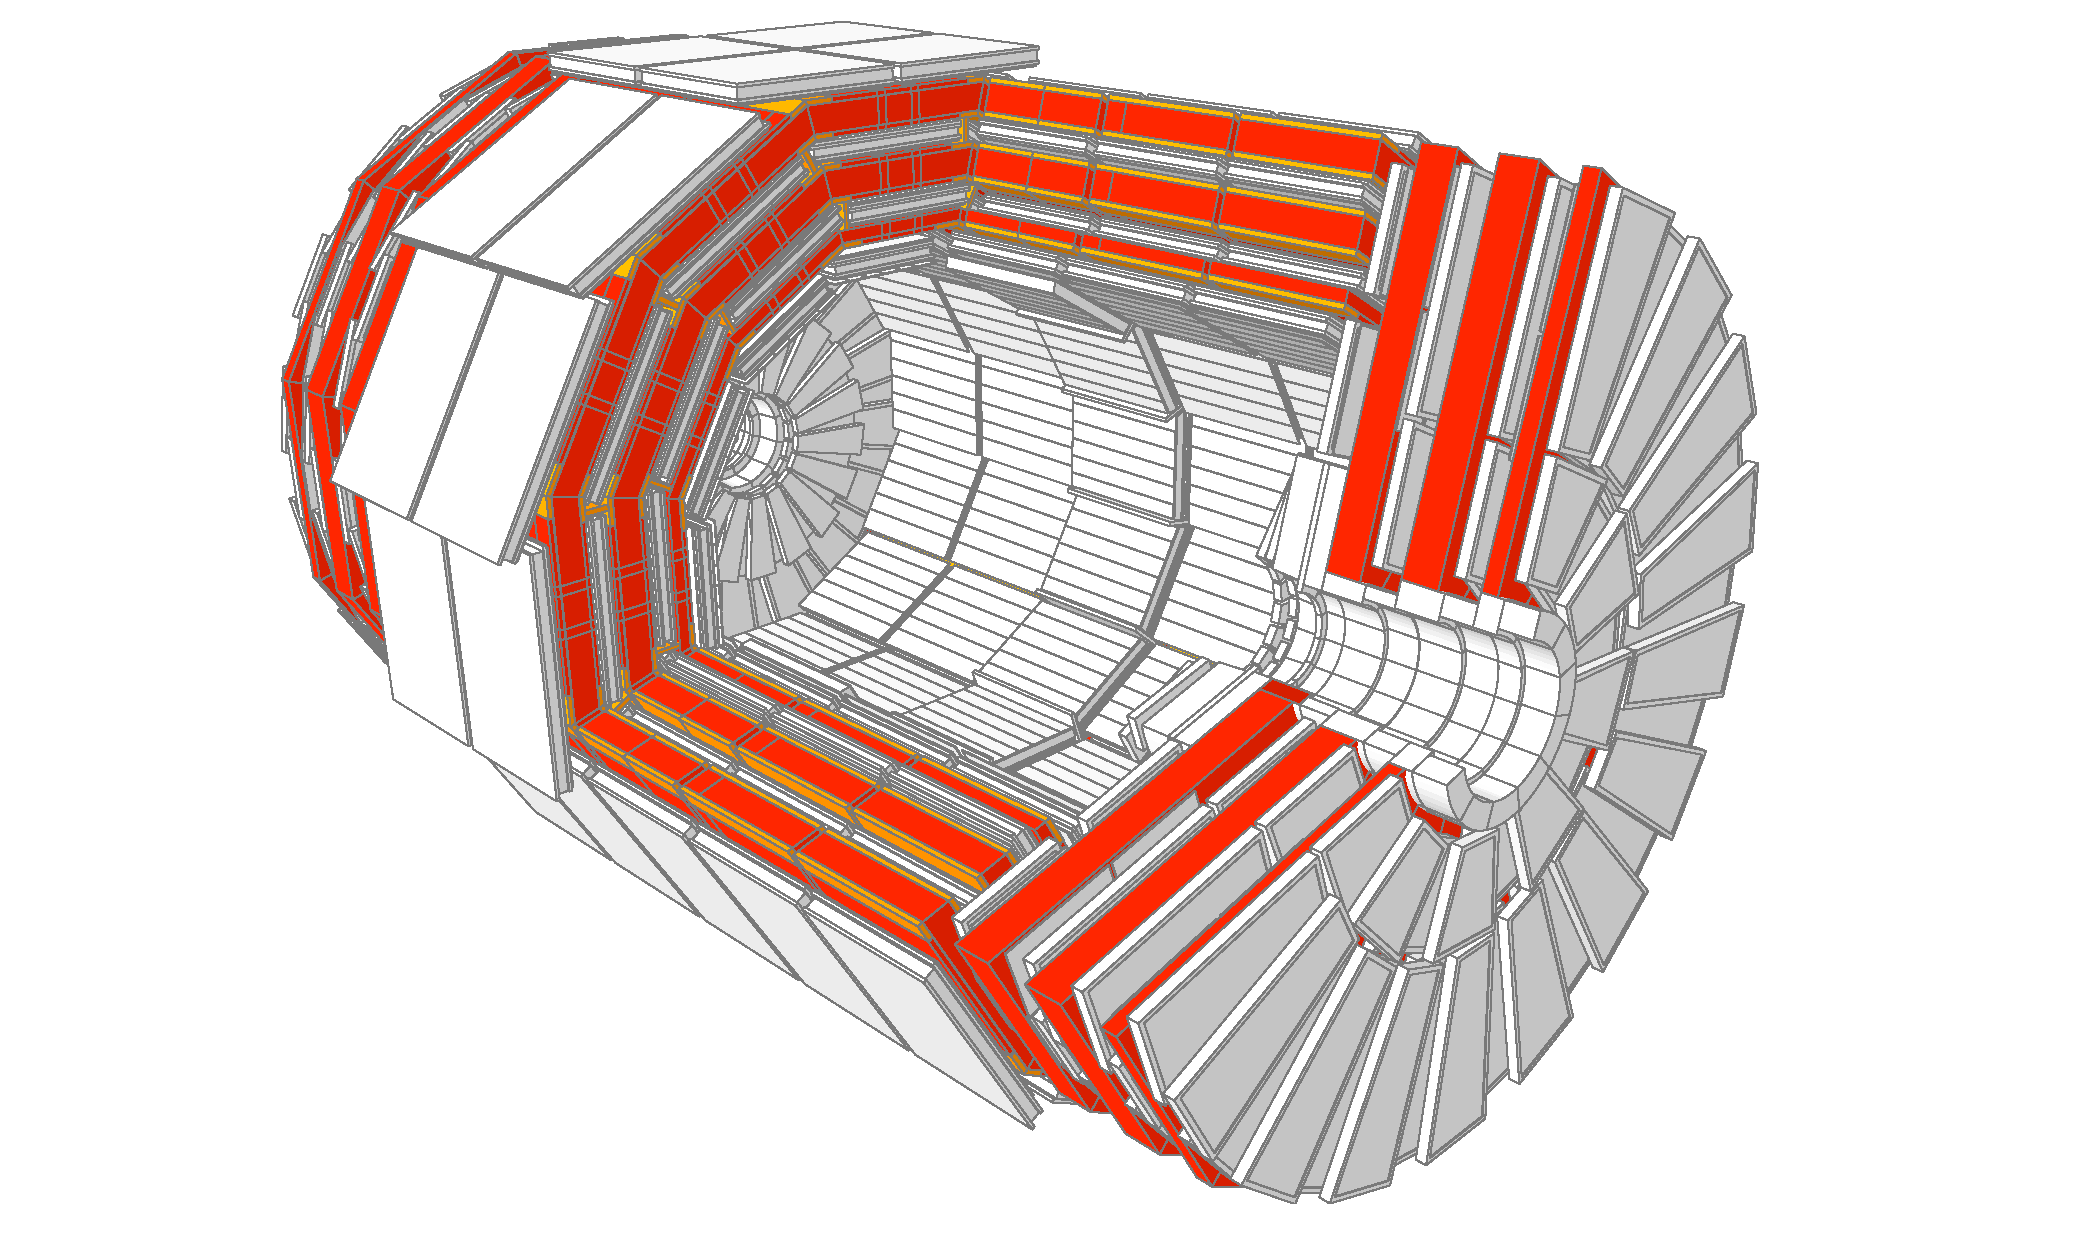
\includegraphics[width=0.49\textwidth]{figures/apparatus/MUON.pdf}
        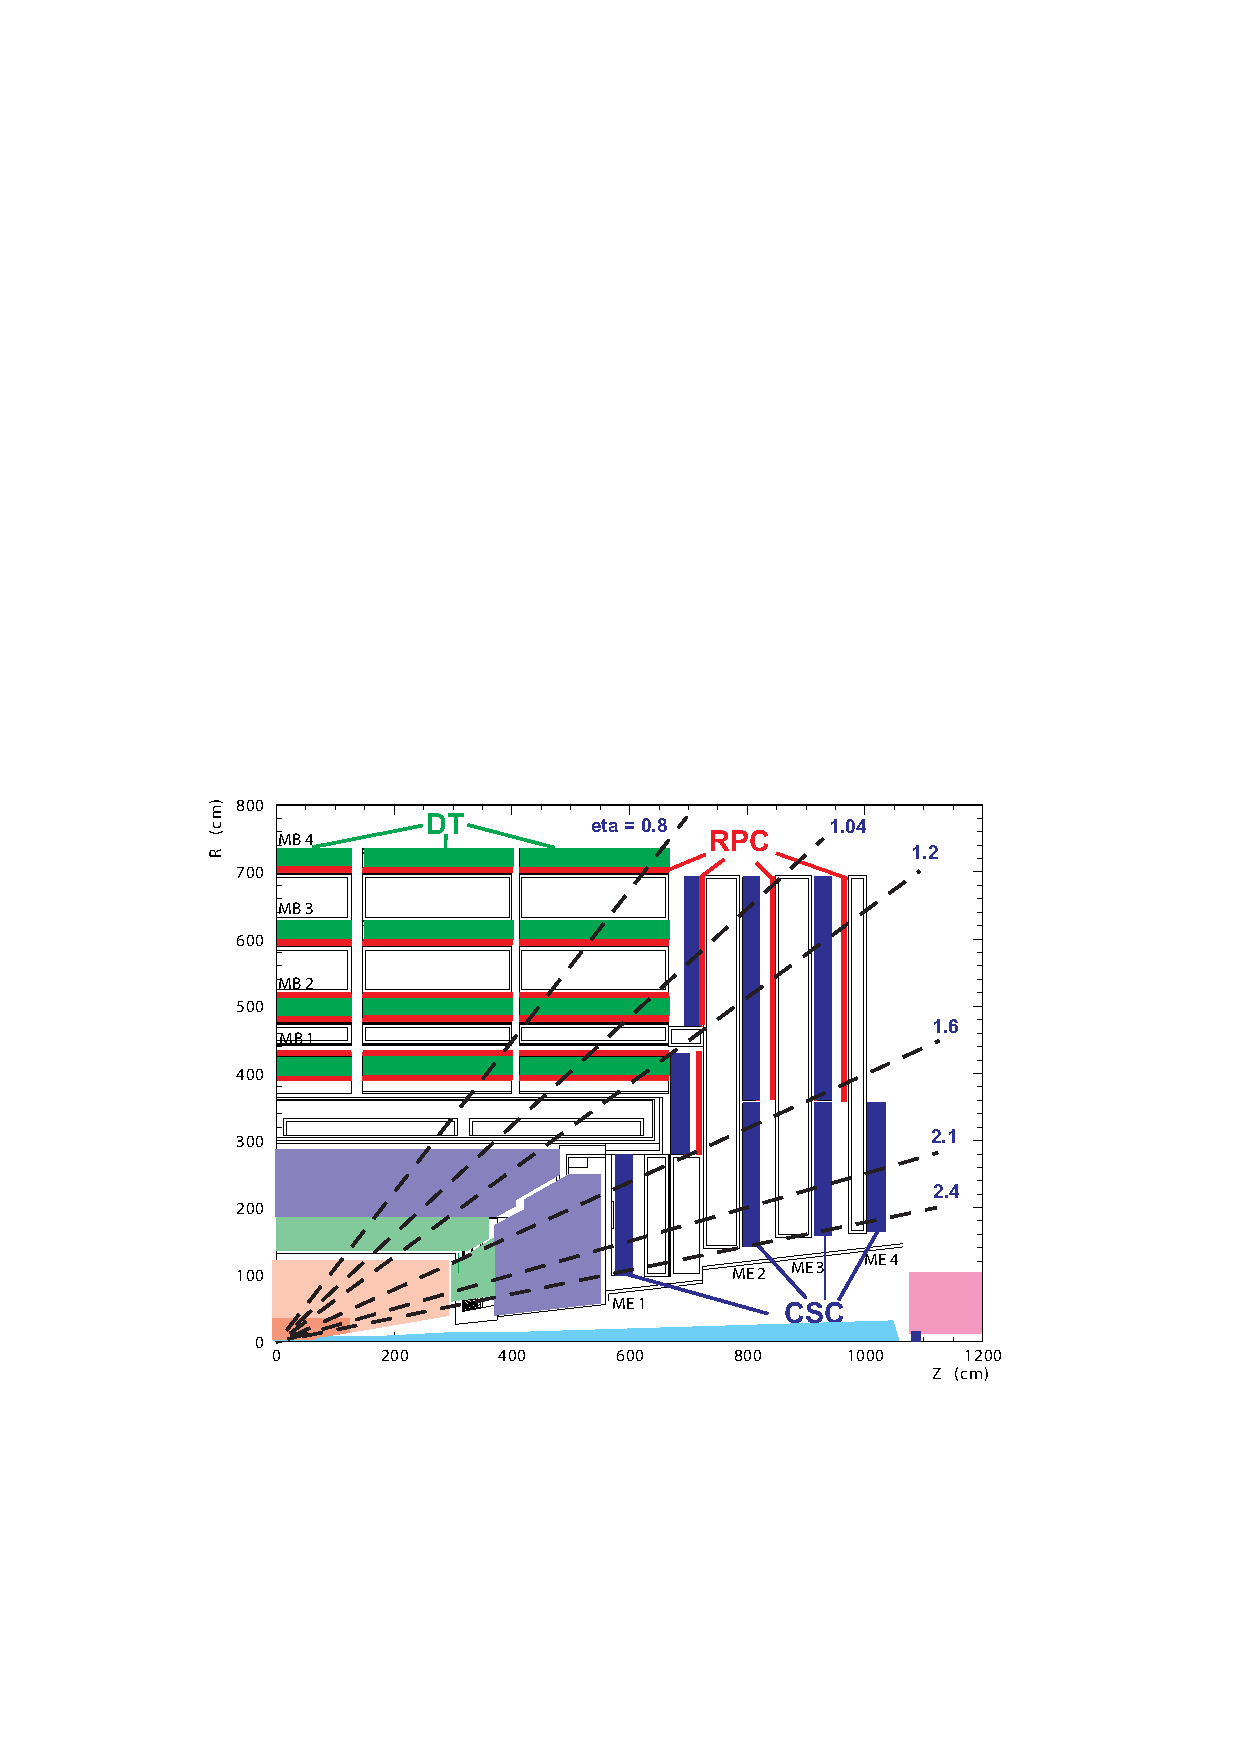
\includegraphics[width=0.49\textwidth]{figures/apparatus/muon_diagram.pdf}
    \end{center}
    \caption{Left: the CMS muon detector subsystems (white) within the structure of the steel return yoke (red) \cite{SketchupCMS}. Right: a diagram showing a quarter-view of of the muon system with detector types labelled.}
    \label{fig:apparatus:muon}
\end{figure}
The muon detectors are all gas-based and belong to three different types: drift tubes (DTs), cathode strip chambers (CSCs) and reactive plate chambers (RPCs). They all operate the same way, with incident particles ionising gas, producing free electrons which drift towards the anode and produce an electrical signal. 

In the barrel region DTs are used as the magnetic field is more uniform, the neutron flux is small and the muon rate is lower. They are arranged in four layers covering the pseudrorapidity $|\eta|<1.2$ where the detectors in the first three layers have a different construction to the fourth. First three layers' detectors consist of 8 chambers in 2 groups of 4: the first half measure in the $r$-$\phi$ plane, the second half measure in $z$. The outermost detectors do not have the $z$ determination. All of these detectors use aluminium wires with an Ar plus CO$_{2}$ gas mix and achieve a position resolution of 100\,$\mu$m.


In the endcap regions the magnetic field is less uniform, the neutron-induced background is high and so is the muon rate. This lead to the adoption of CSC technology due to their fast timing ability, granularity, and robustness to high radiation. 
These detectors cover a pseudorapidity region of $0.9<|\eta|<2.4$ and are arranged in four layers. Each detector consists of 6 gas gaps with cathode strips running radially away from the beamline and anode wires running perpendicularly to the cathode strips. The cathode strips give a precise but relatively slow measurement in the $r$-$\phi$ plane and the anodes measure in $\eta$ with fast timing for triggering and bunch crossing attribution. They achieve a position resolution of around 200\,$\mu$m. 


Finally, in addition to the DTs and CSCs, the muon system uses RPCs placed in the barrel and the endcaps (up to $|\eta|<1.6$) as an independent and complimentary way of triggering. 
RPCs are double gap chambers operating in avalanche mode to give a fast response time and good timing resolution. In the barrel region there are six layers of RPCs: two layers in each of the first two layers of drift tubes and one each in the last two. This redundancy helps with triggering on muons with low-$p_{T}$. In the endcaps there are planes of RPCs in each of the layers that, in addition to triggering, help to resolve ambiguities in the CSCs when there are multiple tracks in a chamber. 


\subsection{Trigger system and Storage}
The LHC delivered bunch crossings to CMS at a rate of 40\,MHz in the 2016 period. With each of these events requiring up to 1MB of memory this would amount 40\,TB per second of readout and storage which is not feasible. 
However, most of these events are not physically interesting: they will mostly be low-energy interactions where the protons only glance off each other rather than collide head-on. 

To filter these events a fast measurement and decision must be made whether to store or discard, this is achieved with the CMS trigger system \cite{trigger}. The trigger system operates as a two-step process: first the hardware-based level-1 trigger (L1T) makes fast decisions on whether to keep events using coarse information from some of the subsystems; and then the software-based high-level trigger (HLT) cuts the rate further by using all detector subsystems and a basic physics object reconstruction. 


The L1T achieves a rate reduction of 40\,MHz to 100\,kHz by performing fast calculations using custom, reprogrammable hardware called field-programmable gate arrays (FPGAs).
To achieve this the L1T must make an accept decision within 3.2\,$\mu$s including time of transmission from the detector and decision return. 
Coarse information is received from the ECAL, HCAL, and the muon system due to speed and bandwidth limitations and stored in a buffer that contains information from multiple bunch crossings. 
Furthermore there is insufficient time for using correlations between subdetectors and also insufficient time and other resources to use information from the tracker. 
Once information is received, a collection of algorithms are used to pick out relevant events and if the event is accepted the entire detector readout is passed on to the HLT.


At the HLT the data rate is still too high and must be cut further to 1\,kHz. This is achieved with a computing farm a short distance away from the CMS detector which runs a basic reconstruction of physics objects from the full CMS readout including the tracker. Here more sophisticated algorithms may be run to pick out collections of objects in events and make the final accept decision.
After this events are recorded to permanent storage, put through the full CMS reconstruction, evaluated for data quality and then made available to physics analyses. 





